
\lhead[]{CAPÍTULO 3. ANÁLISIS DE IDS: ESTADO DEL ARTE}

\section{Introducción}

En el capítulo anterior se introdujo el ámbito de comprensión de programas con las definiciones de los conceptos más importantes. Este capítulo se centra en el estado del arte de algunas técnicas y herramientas orientadas a la CP. Las mismas basan su análisis en los identificadores (ids) situados en los códigos de programas. También se explica de la importancia que tienen los comentarios y los literales al momento de examinar ids. Al final del capítulo se brindan algunos comentarios sobre los temas tratados. A continuación se desarrolla una introducción sobre la temática asociada a identificadores.

Los equipos de desarrollo de software frecuentemente enfocan todo su esfuerzo en el análisis, diseño, implementación y mantenimiento de los sistemas, restándole importancia a la documentación. Por lo tanto, es común encontrar paquetes de software carentes de documentación, lo cual indica que la lectura de los códigos de los sistemas es la única manera de interpretarlos. Es necesaria la interpretación del sistema sobre todo en grandes equipos de desarrollo, por el simple hecho de que un integrante del equipo puede tomar código ajeno para continuar con su desarrollo o realizar algún tipo de mantenimiento.

Teniendo en cuenta que los códigos crecen con los nuevos requerimientos y el frecuente mantenimiento, los sistemas son cada vez más complejos y difíciles de entender. Un camino para lograr un entendimiento ágil y facilitar las arduas tareas de interpretación de códigos, es a través del uso de las herramientas de comprensión. Estas herramientas presentan diferentes perspectivas del sistema, y con esto se agiliza su análisis e inspección. Para diseñar y construir este tipo de herramientas, se recurre al área de CP.
Como se mencionó en el capítulo anterior, la CP es un área de la Ingeniería de Software que brinda métodos, técnicas y herramientas que facilitan al programador entender los programas. Un aspecto importante de la CP es la extracción de información estática (Ver Capítulo 2). El correspondiente trabajo final hará más hincapié en esta temática. Cabe destacar que el resto de las temáticas asociadas a la CP no dejan de ser importantes, sin embargo su análisis escapan a los objetivos de este trabajo.

Una forma de extraer información estática es aplicar técnicas de compilación conocidas, con estas técnicas se extrae información que hay detrás de los componentes visibles en los códigos.
%whats the name - Lawrie
Entre los distintos componentes visibles, los lectores de los códigos fijan su atención principalmente en los ids y los comentarios, ambos son una fuente de información importante para la CP. Sin embargo, cuando en el código no abundan los comentarios, el foco de atención se centra en los ids. 

El la tabla \ref{tabla1} se muestra un análisis léxico que se realizó sobre 2.7 millones de líneas de códigos escritos en lenguaje JAVA \cite{DFPM05,DMDJ13}.

\begin{center}

	\begin{table}[h]	
		\centering
   		\begin{tabular}{| l | c | c | c | c | }  
       
       \hline
  	   \shortstack{\textbf{Elementos de} \\ \textbf{un código}} & \shortstack{\textbf{Cant. por}\\\textbf{elemento}} & \shortstack{\textbf{\% / total de}\\\textbf{elementos}} & \shortstack{\textbf{Caracteres}\\\textbf{utilizados}} & \shortstack{\textbf{\% / total de}\\\textbf{caracteres}} \\ \hline
  	   Palabras claves & 1321005 & 11.2 \% & 6367677 & 12.7 \%\\ \hline
   	   Delimitadores & 5477822 & 46.6 \% & 5477822 & 11.0 \%\\ \hline
       Operadores & 701607 & 6.0 \% & 889370 & 1.8 \%\\ \hline
       Literales & 378057 & 3.2 \% & 1520366 & 3.0 \%\\ \hline          
       \textbf{Identificadores} & 3886684 & 33.0 \% & \textbf{35723272} & \textbf{71.5} \%\\ \hline
       \textbf{Total} & \textbf{11765175} & \textbf{100.0} \% & \textbf{49978507} & \textbf{100.0} \%\\ \hline
     
   	\end{tabular}  
	   
   \caption{Análisis Léxico de códigos JAVA}
   \label{tabla1}
   
  \end{table} 

\end{center}

\vspace{-2.5em}

En la tabla \ref{tabla1} se ve claramente que más de las dos terceras partes (71.5\%) de los caracteres en el código fuente forman parte de un id. 
Por ende, en el ámbito de CP los ids son una fuente importante de información que el lector del código o encargado de mantenimiento debe tener en cuenta. Utilizar una herramienta que analice los ids dando a conocer su significado ayuda a revelar esta información, mejora la comprensión, aumenta la productividad y agiliza el mantenimiento de los sistemas.

Por lo antedicho, construir herramientas de CP que analicen ids en los códigos fuentes de los programas constituye un aporte importante al ámbito de CP. Antes de comenzar con la incursión de herramientas existentes que analizan ids, se detallan algunos conceptos claves relacionados con la temática.

\section{Conceptos claves}

\textit{“Un \textbf{Identificador (id)} básicamente se define como una secuencia de letras, dígitos o caracteres especiales de cualquier longitud que sirve para identificar las entidades del programa”}
 
Cada lenguaje tiene sus propias reglas que definen cómo pueden estar construidos los nombres de sus ids. Por ejemplo, en JAVA no está permitido declarar ids que coincidan con palabras reservadas o que contengan operadores relacionales o matemáticos ($+$ $-$ $\&$ $!$ $\%$), a excepción del guión bajo (\_ ) o signo peso (\$). Ejemplo: \textsf{var\_char, var\$char}.

%whats the name - Lawrie
%Para mejorar la CP se requiere que los nombres de los ids comuniquen de manera clara los conceptos que representan. Sin embargo, en la práctica no se tiene muy en cuenta. 
Generalmente, la buena práctica de programación recomienda que al momento de construir un id dentro del código, el mismo debe estar asociado a un concepto \cite{DFPM05,DMDJ13,LDFHB07}.

\begin{center}
\textsf{Identificador $\Leftrightarrow$ Concepto}
\end{center}

%Dicho de otra manera un id es un representante de un concepto ubicado en el dominio del problema.
%Por ejemplo, el id \textsf{openWindow} está asociado al concepto `abrir una ventana'.
Por ejemplo, el id \textsf{userAccount} está asociado al concepto `cuenta de usuario', en este caso si el sistema que se analiza es bancario, el concepto antedicho pertenece al Dominio del Problema. Por lo tanto, uno de los requisitos importantes que debe reunir un programa para facilitar su comprensión es que sus ids sean claros, de esta manera se podrán ver más fácilmente los conceptos que cada id representa. Sin embargo, dicho requerimiento no es tenido muy en cuenta por los programadores \cite{DFPM05,DLHD06,DCHD06,LDFHB07}.

En la siguiente sección se menciona, cómo los nombres asignados a los ids impacta enormemente en la interpretación del concepto que el id tiene asociado, por lo tanto afecta la lectura comprensiva del código. Todas estas características, son tenidas en cuenta en el ámbito de la CP.


\section{Nombres de Identificadores}

%Deißenbock and Pizka DFPM05
%Intro
Durante el desarrollo del sistema, las reglas de construcción de ids se enfocan más en el formato del código y el formato de la documentación, en lugar de enfocarse en el concepto que el id representa. Más adelante de la etapa de desarrollo, viene la etapa de mantenimiento del sistema, aquí es probable que el encargado de hacerlo, no sea el mismo que desarrolló el sistema y generalmente no tiene en cuenta los nombres de los ids, ni que conceptos representan a la hora de interpretar el código.

%También durante la etapa de mantenimiento del software la forma en la que los ids están nombrados no es muy tenida en cuenta para comprender el sistema. 

Antes de proseguir sobre la importancia que tienen los nombres de los ids en la CP, a continuación se clasifican las distintas formas que se puede nombrar un id multi-palabra\footnote[1]{Que contiene más de una palabra.}.

\subsection{Clasificación}
\label{sec:clasif}%para hacer referencia en el cap 4

Estudios realizados con 100 programadores \cite{DCHD06,LDMCFH07} sobre comprensión de ids indican que existen tres formas principales de construir ids multi-palabras (tomando como ejemplo el concepto \textsf{File System Input}): 

\begin{itemize}
\itemsep0em%reduce espacio
\item Palabras completas (\textsf{fileSystemInput}).
\item Abreviaturas (\textsf{flSysIpt}).
\item Una sola letra\footnote[2]{Esta clasificación se la conoce como acrónimo.} (\textsf{fsi}). 
\end{itemize}

También pueden existir la combinación entre dos tipos de clasificaciones: por ejemplo \textsf{flSystemIpt}.

Los estudios antes mencionados le posibilitaron a los investigadores concluir que las palabras completas son las más comprendidas, sin embargo las estadísticas marcan en algunos casos que las abreviaturas que se ubican en segundo lugar, no demuestran una diferencia notoria con respecto a las palabras completas \cite{DCHD06,SBMJ10}.

Los investigadores Feild, Binkley, Lawrie \cite{FBL06,HDD06,BMDDL09,DMDJ13}, clasifican los nombres de los ids con dos términos conocidos en la jerga del análisis de ids: \textit{hardwords} y \textit{softwords}.

Los \textit{hardwords} destacan la separación de cada palabra que compone al id multi-palabra a través de una marca específica; algunos ejemplos son: \mbox{\textsf{fileSystem}} en donde se marca bien la separación de cada palabra con el uso de mayúscula entre las minúsculas\footnote[1]{Este caso es conocido como camel-case ya que las letras en mayúsculas se asemejan a las jorobas de un camello.}, o todas mayúsculas seguidas de todas minúsculas \mbox{\textsf{FILEsystem}}. También se utilizan para dividir las palabras, un símbolo especial, como es el caso del guión bajo: \textsf{file\_system}. 

En cambio los \textit{softwords} no poseen ningún tipo de separador o marca que de indicios de las palabras que lo componen; por ejemplo: \textsf{textinput} o \mbox{\textsf{TEXTINPUT}} que está compuesto por \textsf{text} y por \textsf{input} sin tener una marca que destaque la separación.
La nomenclatura de \textit{hardwords} y \textit{softwords} se utilizará en el resto de este trabajo final. 

Habiendo explicado algunas clasificaciones en lo que respecta al tipo de nombres asignados en los ids, en la próxima sección se retoma la importancia que tienen los nombres utilizados en los ids.

%Si bien en el párrafo anterior se dio una taxonomía de como se clasifican los ids, en los ejemplos no se refleja como normalmente se nombra un id.
%Generalmente los programadores para reducir el esfuerzo de tipeo escriben los ids en forma abreviada compuestos por mas de una palabra, esto se lo conoce con el nombre de acrónimos. Para dar un ejemplo sobre esto: el id \textsf{fileSystem} los programadores lo suelen nombran como \textsf{flSys}, \textsf{fiStm}, \textsf{fl\_sys} u otras tantas posibles representaciones abreviadas.

%Caprile and Tonella state that “identifier names are one of the most important sources of information about program entities”\cite{BCPT00}

%Caprile and Tonella - Software entities are born and live with their names. \cite{BCPT99}

%================================
\subsection{Importancia en los Nombres}
En la actualidad existen innumerables convenciones en cuanto a la construcción sintáctica de los ids, alguno de ellos son:

\begin{itemize}
\itemsep0em%reduce espacio
\item En el caso de JAVA, los nombres de los paquetes deben ser con minúscula (main.packed). Las clases con mayúscula en la primer letra de cada palabra que compone el nombre (MainClass).

\item En el caso de C\#, las clases se nombran igual que JAVA. Pero para el caso de los paquetes deben comenzar con mayúscula y el resto minúscula (Main.Packed).
\end{itemize}

Lo mencionado en los ítems precedentes, indica que se concentra más en los aspectos sintácticos del id y no tanto en los aspectos semánticos, a la hora de asignar nombres a los ids.

%Las investigaciones realizadas por Deissenboeck y Pizka \cite{DFPM05} a este problema parte de que cada nombre de id está asociado a un concepto del dominio del problema y viceversa. 
%Mas formalmente se puede ver como una función biyectiva:

%\begin{center}
%\textsf{Nombre $\Leftrightarrow$ Concepto}
%\end{center} 

%En este contexto se dice que se logra un nombramiento conciso y consistente de ids.

\begin{figure}[t] %[h] para here [b] para bottom [t] para top
\centering
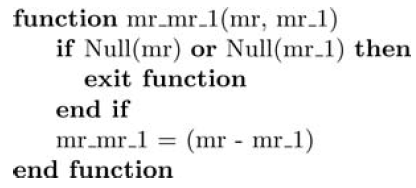
\includegraphics[scale= 0.70]{./cap3/idd_1.png}
\caption{Trozo de Código de un Sistema Comercial}
\label{captura2}
\end{figure}

%Problema: de porque no existe un correcto nombramiento
Una evidencia fehaciente de la importancia en la semántica de nombres, son las técnicas que se aplican para protección de código. Algunas de ellas se encargan de reemplazar los nombres originales de los ids por secuencias de caracteres aleatorios y de esta manera se reduce la comprensión. Estas técnicas se conocen con el nombre de ofuscación de código. La ofuscación es común en los sistemas de índole comercial, en la Figura \ref{captura2} se puede observar un ejemplo tomado de un caso real, en donde la función \textsf{mr\_mr\_1} no parece complicada pero se desconoce la finalidad de su ejecución \cite{DFPM05}.

A su vez, los programadores cuando desarrollan sus aplicaciones, restan importancia a la semántica de nombres asignados a los ids. Existen tres razones destacadas que conllevan a esto:

\begin{enumerate}
\itemsep0em%reduce espacio
\item Los ids son escogidos por los programadores, sin tener en cuenta los conceptos que tienen asociados.

\item Los desarrolladores tienen poco conocimiento de los nombres usados en los ids ubicados en otros sectores del código fuente.

\item Durante la evolución del sistema, los nombres de los ids se mantienen y no se adaptan a nuevas funcionalidades (o conceptos) que puedan tener asociado.
\end{enumerate}

En este sentido, la construcción de ids poco claros, se combate con la programación “menos egoísta”. Esta consiste en hacer programas más comprensibles para el futuro lector que no está familiarizado con el código. Para lograrlo se deben respetar dos reglas sobre los nombres que se le asignan a los ids \cite{DFPM05,DLHD06}:

%\noindent remueve la sangria!
\begin{framed}
\noindent \textbf{Nombre Conciso:} El nombre de un id es conciso, si la semántica del nombre coincide exactamente con la semántica del concepto que el id representa.

\noindent \textbf{Nombre Consistente:} Cada id, debe tener asociado si y solo si, un único concepto (relación biyectiva entre los ids y los conceptos).
\end{framed}

Un ejemplo de \textit{conciso} es \textsf{output\_file\_name} que representa el concepto de `nombre de archivo de salida', distinto sería un id nombrado como \textsf{file\_name}, el cual está incompleto y no representa de forma semánticamente concisa el concepto mencionado.

%sinonimos y homonimos
Los propiedades que violan nombrar a un id de manera \textit{consistente} son conocidas en el lenguaje natural como sinónimos y homónimos. 
Los homónimos son palabras que pueden tener más de un significado. Por ende, si el nombre de un id está asociado a más de un concepto, no estará claro que concepto representa. Por ejemplo, un id con el nombre \textsf{file} generalmente se asocia al concepto de `archivo', pero puede que se refiera a una estructura del tipo cola.

Por otro lado, los sinónimos indican que para un mismo concepto pueden tener asociados diferentes nombres. Por ejemplo, un id con el nombre \mbox{\textsf{accountBankNumber}} y otro \textsf{accountBankNum} son sinónimos porque hacen referencia al mismo concepto `número de cuenta bancaria'. 

Esta demostrado \cite{DFPM05,DLHD06,NIATL98,DMDJ13} que la ausencia de nombres consistentes tales como se mencionó anteriormente, hacen que se dificulte identificar con claridad los conceptos en el dominio del problema, lo que hace aumentar los esfuerzos de comprensión del programa. 


Por lo tanto, si los ids están construidos de forma \textit{concisa} (identificando bien al concepto) y la \textit{consistencia} está presente, se pueden descubrir los conceptos que representan en el dominio del problema más fácilmente. De esta manera, se agiliza la comprensión, aumenta la productividad, mejora la calidad durante la etapa de mantenimiento \cite{DFPM05,DLHD06}.%agregar mas bibliografia

Intuitivamente, se necesita que los ids representen bien al concepto, ya que mayor será el impacto que tendrá en la interpretación del sistema \cite{DFPM05,DLHD06,SBWYY10}. Sin embargo, durante las etapas de desarrollo y mantenimiento de software, es muy difícil mantener una consistencia global de nombres en los ids, sobre todo si el sistema es grande. En este sentido, cada vez que un concepto se modifica el nombre del id asociado debe cambiar y adaptarse a la modificación.

%solucion propuesta
Los autores Deissenboeck y Pizka \cite{DFPM05} elaboraron una herramienta que ayuda a la construcción y mantenimiento de ids con nombres concisos y consistentes. Dada la dificultad que conlleva construir una herramienta totalmente automática que se encargue de nombrar y mantener correctamente los ids, ellos elaboraron una herramienta que necesita la intervención del programador. Esta herramienta, a medida que el sistema se va desarrollando, construye y mantiene un diccionario de datos compuesto con información de ids. En el ámbito de la Ingeniería de Software el concepto de diccionarios de datos es importante.


\begin{description}
\item[Diccionarios de Datos:] Este concepto conocido también como `glosario de proyecto' se recomienda en los textos orientados a la administración de proyectos de software. Con los diccionarios se describe en forma clara todos los términos utilizados en los grandes sistemas de software. También brindan una referencia completa a todos los participantes de un proyecto durante todo el ciclo de vida del producto \cite{RSPMGH02}.
\end{description}

Este concepto sirvió de inspiración a los autores para construir la herramienta, que a continuación se describe.

\begin{figure}[t!] %[h] para here [b] para bottom [t] para top
\centerline{%queda centrada mejor la imagen
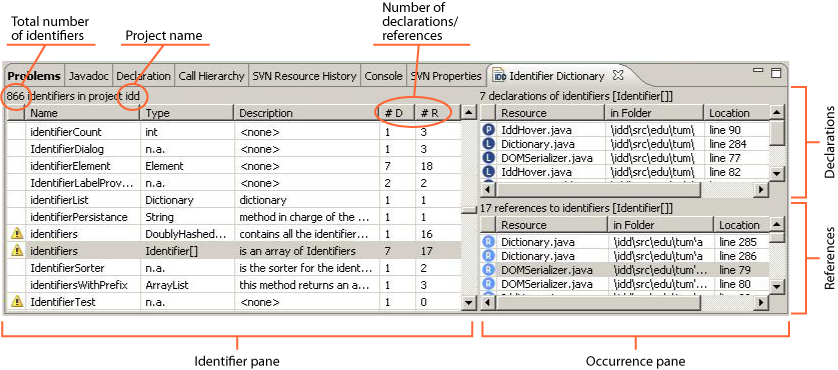
\includegraphics[scale= 0.55]{./cap3/idd_2.png}
}
\caption{Visualización de Identifier Dictionary}
\label{captura3}
\end{figure}

\pagebreak
\subsection{Herramienta: Identifier Dictionary}
\label{sec:algIdDic}
La herramienta conocida con el nombre de \textit{Identifier Dictionary} (IDD)\footnote[1]{http://www4.informatik.tu-muenchen.de/\~{}ccsm/idd/index.html} construida por Deissenboeck y Pizka \cite{DFPM05} actúa como un diccionario de datos, que ayuda al desarrollador a mantener la consistencia de nombres en los ids de un proyecto JAVA. Es una base de datos que almacena información de los ids tales como el nombre, el tipo del objeto que identifica y una descripción comprensiva.

La herramienta IDD ayuda a reducir la creación de nombres sinónimos (Ver apartado anterior) y asiste a escoger un nombre adecuado para los ids siguiendo el patrón de nombres existentes. Además, aumenta la velocidad de comprensión del código en base a las descripciones de cada id. El equipo encargado de tareas de mantenimiento localiza un concepto del dominio del problema y luego su correspondiente id de manera ágil. Otro aporte que hace la herramienta es asegurar la calidad de los nombres (nombres concisos) de los ids con un esfuerzo moderado, usando como ayuda la descripción comprensiva ubicada en la base de datos \cite{DFPM05,LFBEX07}.

Se implementó como extensión de la IDE Eclipse 3.1\footnote[2]{http://www.eclipse.org/jdt}. Se visualiza en el panel de las vistas de la IDE y consiste de tres secciones (Ver Figura \ref{captura3}):

\begin{figure}[t] %[h] para here [b] para bottom [t] para top
\centerline{%queda centrada mejor la imagen
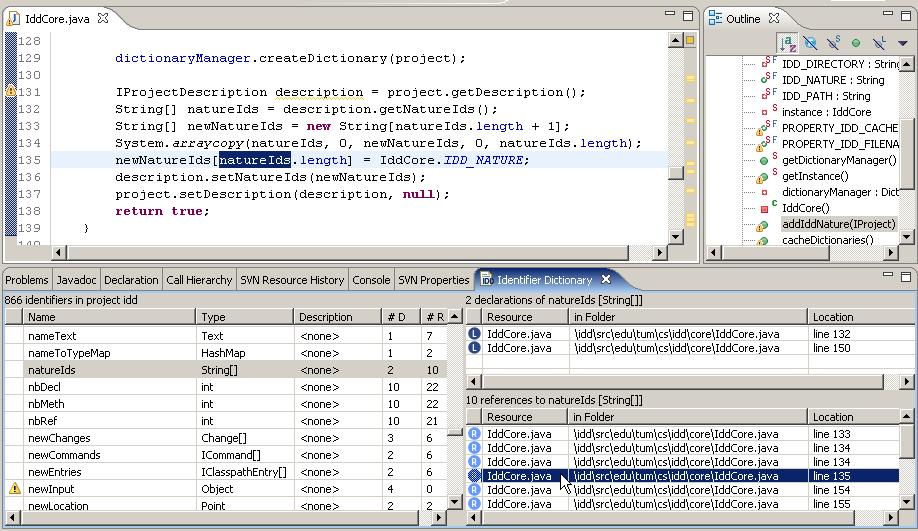
\includegraphics[scale= 0.50]{./cap3/idd_3.png}
}
\caption{Visualización de Identifier Dictionary}
\label{captura4}
\end{figure} 

\begin{itemize}
\itemsep0em%reduce espacio
\item Una tabla con información de los ids en el proyecto: nombre, tipo, descripción, cantidad de declaraciones y cantidad de referencias (Identifier pane).
\item Una lista de ids declarados en el proyecto (Ocurrence pane).
\item Una lista de referencias de los ids en el proyecto (Ocurrence pane).
\end{itemize}

Mientras se realiza el desarrollo del código la herramienta asiste al programador a llevar buenas prácticas de asignación de nombres en los ids, a través de las siguientes características:

\textbf{Navegación en el código fuente:} Si se selecciona un id, en la tabla de ids (inferior izquierda), mostrará la ubicación exacta en donde se encuentra cada declaración y referencia (Ver Figura \ref{captura4}).

%\begin{figure}[h] %[h] para here [b] para bottom [t] para top
%\centering
%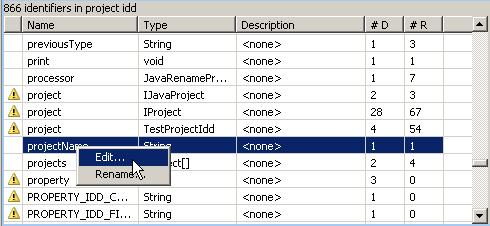
\includegraphics[scale= 0.55]{./cap3/idd_4.png}
%\caption{Visualización de Identifier Dictionary}
%\label{captura5}
%\end{figure}
%
%\textbf{Guardar descripción:} Botón derecho en el panel de ids y luego en edit. Permite agregar una descripción comprensiva (Figura \ref{captura5}).

%\begin{figure}[h] %[h] para here [b] para bottom [t] para top
%\centering
%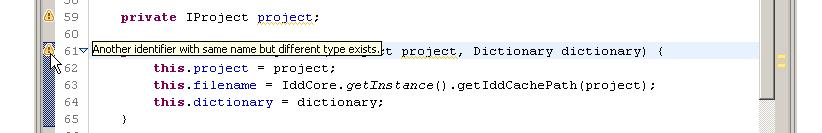
\includegraphics[scale= 0.55]{./cap3/idd_5.png}
%\caption{Visualización de Identifier Dictionary}
%\label{captura6}
%\end{figure}
\begin{figure}[t] %[h] para here [b] para bottom [t] para top
\centerline{%queda centrada mejor la imagen
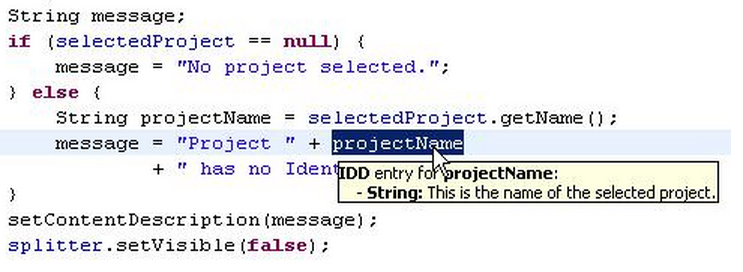
\includegraphics[scale= 0.70]{./cap3/idd_7.png}
}
\caption{Visualización de Identifier Dictionary}
\label{captura8}
\end{figure}

\textbf{Advertencias (warnings):} Mientras se realiza la recolección de ids, los íconos de advertencia indican potenciales problemas en el nombre asignado.  Los dos tipos de mensajes que se muestran son: dos ids con el mismo nombre pero distinto tipos y el id es declarado pero no referenciado\footnote[1]{Similar a los warnings de Eclipse}.

%\begin{figure}[h] %[h] para here [b] para bottom [t] para top
%\centering
%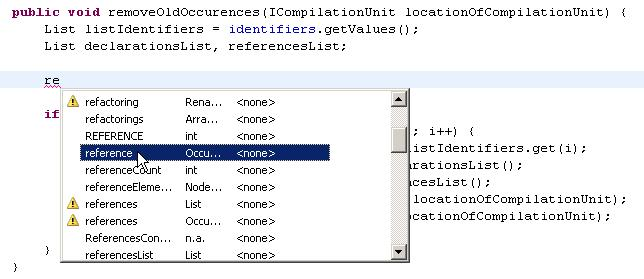
\includegraphics[scale= 0.55]{./cap3/idd_6.png}
%\caption{Visualización de Identifier Dictionary}
%\label{captura7}
%\end{figure}

\textbf{Mensajes pop-up:} Se puede visualizar información tales como: la descripción del id mientras se está programando, esto se logra posicionando el cursor sobre el id en el código fuente (Ver Figura \ref{captura8}).

\textbf{Auto-completar nombres:} Las IDE\footnote[2]{Entornos de desarrollos integrados, por su siglas en inglés. Netbeans, Eclipce etc.} actuales proveen la función de auto-completar.
Sin embargo, esta funcionalidad falla cuando los nombres de los ids no están declarados dentro del alcance actual de edición. Con el plugin IDD a la hora de auto-completar mira todos los ids del proyecto sin importar el ambiente en el que se encuentre.

\textbf{Renombre global de ids:} Esta función permite renombrar cualquier id generando una vista previa y validando el nombre de los ids a medida que el sistema va evolucionando. De esta forma se preserva la consistencia global de nombres.

La herramienta IDD trabaja internamente con un colector de ids que está acoplado al proceso de compilación del proyecto (Build Proyect) de Eclipse. Los ids se van recolectando a medida que el programa se va compilando. Los nombres, el tipo, la descripción se van guardando en un archivo XML. También se puede exportar en un archivo en formato HTML el cual permite una lectura más clara de los ids con toda información asociada \cite{DFPM05}.


%%=========Lawrie

La herramienta IDD colabora en mejorar los nombre de los ids con un esfuerzo moderado como se describió antes.
Sin embargo, los investigadores Feild, Binkley, Lawrie \cite{LFBEX07,DLHD06} determinaron que en IDD, los esfuerzos son moderados solo para sistemas que se empiezan a programar desde el comienzo y no con sistemas ya existentes.

Para concluir con esta sección, la buena calidad en los nombres de los ids mejora el entendimiento del código. Además, muchos expertos sostienen que las técnicas de Ingeniería Inversa se emplean con mayor precisión si el código está bien escrito. Algunas de estas técnicas tienen como objetivo mejorar la CP, y una forma conocida de lograrlo es traduciendo los nombres abreviados de los ids a palabras más completas en lenguaje natural. En la siguiente sección se describen este tipo de técnicas de regresión.

%%=====================================

\section{Traducción de Identificadores}
\label{sec:tradIdDicc}%para hacer referencia en el cap 4

Los lectores de códigos de programas tienen inconvenientes para entender el propósito de los ids y deben invertir tiempo en analizar el significado de su presencia. Por esta razón, las estrategias automáticas dedicadas a facilitar este análisis son bienvenidas en el contexto de la CP.

Para aliviar el inconveniente mencionado anteriormente, un camino viable, consiste en descubrir la información que ocultan los ids detrás de sus abreviaturas. Esta información es relevante ya que pertenece al dominio del problema \cite{EHPV09,LFBEX07}. 

\subsection{Conceptos y Desafíos observados}

Una manera de descubrir la información oculta detrás de los ids, es intentar convertir estas abreviaturas en palabras completas del lenguaje natural. Por ende, el foco del análisis de los ids se basa en la traducción de palabras abreviadas a palabras completas.

El proceso que se encarga de realizar la traducción de ids consta de dos pasos \cite{LFBEX07}:

\begin{enumerate}
\itemsep0em%reduce espacio
\item \textbf{División:} Separar el id en las palabras que lo componen usando algún separador especial\footnote[1]{Siempre y cuando el id sea multi-palabra (contenga más de una palabra).}. (Ejemplo: \textsf{flSys} $\Rightarrow$ \textsf{fl-sys}).

\item \textbf{Expansión:} Expandir las abreviaturas que resultaron como producto del paso anterior. (Ejemplo: \textsf{fl-sys} $\Rightarrow$ \textsf{file system}).
\end{enumerate}

Cabe mencionar que el ejemplo mostrado en ambos pasos corresponde a un caso de \textit{hardword} en donde la separación de las palabras es destacada. Sin embargo, la dificultad se presenta en los \textit{softwords} (Ver sección anterior) ya que la división no está marcada (Ejemplo: \textsf{hashtable} $\Rightarrow$ \textsf{hash-table}). Existen también casos híbridos (Ejemplo: \textsf{hashtable\_entry}). En este caso el id tiene una marca de separación (guión bajo) con dos hardwords \textsf{hashtable} y \textsf{entry}. A su vez el hardword \textsf{hashtable} posee dos softwords \textsf{hash} y \textsf{table}, mientras que \textsf{entry} es un hardword compuesto por un único softword.

%noindent - Elimina sangria
\begin{framed}
\noindent El principal desafío (y el más complejo) en la traducción de ids, es detectar los casos de \textit{softword}. Luego proceder a separar las palabras abreviadas que la componen para posteriormente realizar la expansión \cite{FBL06,LFBEX07}.  
\end{framed}

Para afrontar este objetivo los especialistas deciden recurrir a fuentes de palabras en lenguaje natural. Existen 2 tipos de fuentes, dentro del mismo código extrayendo palabras presentes en comentarios, literales y documentación. La otra fuente se encuentra fuera del programa consultando diccionarios o listas de palabras predefinidas. 

Habiendo explicado el proceso encargado de expandir las abreviaturas de un id a palabras completas, el siguiente paso es describir las herramientas conocidas que lo implementan. 

La autora Emily Hill \cite{EZH08} con alto reconocimiento por su investigación en lo que respecta a expandir ids en códigos JAVA, explica algunas amenazas y desafíos a tener en cuenta a la hora de desarrollar herramientas que analizan ids. A continuación se explican algunas de ellas.

\begin{description}
\itemsep0em%reduceenglish espacio
\item[Dificultad para armar diccionarios apropiados:]  La mayoría de los diccionarios, se usan para corregir la ortografía. Las palabras que incluyen son sustantivos propios, abreviaturas, contracciones\footnote[1]{Palabras en inglés que llevan apostrofes, ejemplo: let's.} y demás palabras que puedan aparecer en un software. Sin embargo, la inclusión de muchas palabras genera que una simple abreviatura (\textit{char, tab, id}) se trate como una palabra expandida y no se expanda. Por el contrario, si el diccionario contiene pocas palabras, la expansión se realiza más frecuente de lo normal.
% lo ideal es disponer de un diccionario con palabras que incluyan solo palabras adecuadas al ámbito de la ciencias de la computación pero lamentablemente esto no está disponible.

\item[Dificultad para traducir abreviaturas cortas:] Si un id está 
abreviado como `\textsf{def}', es complicado determinar con precisión cual es la mejor traducción entre tantos candidatos \textsf{definition, default, defect}. Otra observación hecha, es que mientras más corta es la abreviatura más candidatos posee, el ejemplo más común es \textsf{i} que generalmente es \textsf{integer} pero podrían ser otros tantos \textsf{interface, interrupt}, etc. Se requieren procesos inteligentes para solucionarlo.

\item[Distintas políticas de expansión:] Si la abreviatura se mira como prefijo tiene menos candidatos a traducirse, un ejemplo es `\textsf{str}' el cual coincide con \textbf{STR}\textsf{ing}, \textbf{STR}\textsf{eam}. En cambio si las letras de \textsf{str} forman parte de la palabra tiene más posibilidades de expansión \textbf{S}\textsf{ubs}\textbf{TR}\textsf{ing}, \textbf{ST}\textsf{o}\textbf{R}\textsf{e}, \textbf{S}\textbf{ep}\textbf{T}\textbf{embe}\textbf{R}, \textbf{S}\textbf{a}\textbf{T}\textbf{u}\textbf{R}\textbf{n}.
\end{description}

Las palabras abreviadas, usadas en los ids dependen mucho de la idiosincrasia del programador. Por lo tanto, construir herramientas automáticas que analicen ids representa un verdadero desafío en el área de CP.

En las próximas dos secciones se explican algoritmos encargados de la división de ids, y en la secciones subsiguientes se describen algoritmos de expansión. En todos los casos se presentan pseudo-códigos de los algoritmos que ejecuta cada técnica, de esta manera ayudarán al lector a entender el funcionamiento de cada una.

%Se puede usar técnicas de recuperación de información para mejorar el procedimiento de traducción.

%greedy - samurai 
\subsection{Algoritmo de División Greedy}
\label{sec:algGre}

El Algoritmo de división Greedy elaborado por Lawrie, Feild, Binkley \cite{DLFB06,FBL06,HDD06,LFBEX07,EHPV09}, emplea tres listas para realizar su trabajo:

\begin{description}
\itemsep0em%reduce espacio
\item[Palabras de diccionarios:] Contiene palabras de diccionarios públicos y del diccionario que utiliza el comando de Linux \textsf{ispell}\footnote[1]{Comando de Linux generalmente utilizado para corregir errores ortográficos, en archivos de texto. http://wordlist.aspell.net}.

\item[Abreviaturas conocidas:] La lista se arma con abreviaturas extraídas de distintos programas y de autores expertos. Se incluyen abreviaturas comunes (ejemplo: \textsf{alt} $\Rightarrow$ \textsf{altitude}) y abreviaturas de programación (ejemplo: \textsf{txt} $\Rightarrow$ \textsf{text}).

\item[Palabras excluyentes (stop list):] Posee palabras que son irrelevantes para realizar la división de los ids. Incluye palabras claves (ejemplo: \texttt{while}), ids predefinidos (ejemplo: \texttt{NULL}), nombres y funciones de librerías (ejemplo: \texttt{strcpy}, \texttt{errno}), y todos los ids que puedan tener un solo caracter.
\end{description}


\begin{algorithm}[b!]%H fuerza que se genere aqui
\LinesNumbered%enumera las lineas
\SetKwInOut{Input}{Entrada}\SetKwInOut{Output}{Salida}
\SetKwInOut{Global}{Var Global}
\Global{\textit{\textbf{ispellList}} \tcp{\textit{Palabras de ispell + Diccionario}}}
\Global{\textit{\textbf{abrevList}} \tcp{\textit{Abreviaciones conocidas}}}
\Global{\textit{\textbf{stopList}} \tcp{\textit{Palabras Excluyentes}}}
\Input{\textit{\textbf{idHarword}} \tcp{\textit{identificador a dividir}}}
\Output{\textit{\textbf{softwordDiv}} \tcp{\textit{id separado con espacios}}}

\BlankLine
\textit{\textbf{softwordDiv}} $\leftarrow$ “”

\textit{\textbf{softwordDiv}} $\leftarrow$ dividirCaracteresEspecialesDigitos(\textit{\textbf{idHarword}})

\textit{\textbf{softwordDiv}} $\leftarrow$ dividirCamelCase(\textit{\textbf{softwordDiv}})

\BlankLine
\ForAll{$($\textit{\textbf{s}} $|$ \textit{\textbf{s}} es un substring separado por ` ' en \textit{\textbf{softwordDiv}}$)$}{
\BlankLine

\If{$($\textbf{s} no pertenece a $($\textit{\textbf{stopList}} $\cup$ \textit{\textbf{abrevList}} $\cup$ \textbf{ispellList} $))$}{
\BlankLine
resultadoPrefijo $\leftarrow$ buscarPrefijo(\textit{\textbf{s}},“”)

resultadoSufijo $\leftarrow$ buscarSufijo(\textit{\textbf{s}},“”)
\BlankLine
\tcp{\textit{Se elije la división que mayor particiones hizo.}}
\textit{\textbf{s}} $\leftarrow$ maxDivisión(resultadoPrefijo,resultadoSufijo)

}
}
\BlankLine
\Return \textit{\textbf{softwordDiv}} \tcp{\textit{Retorna el id dividido por ` '}}

\caption{División Greedy\label{GSA}}
\end{algorithm}



El algoritmo de Greedy utiliza las 3 listas nombradas al comienzo de la sección en forma de variable global. Esto ocurre porque las 3 listas son usadas por subrutinas más tarde. El algoritmo procede de la siguiente manera (Ver Algoritmo \ref{GSA}), el id que recibe como entrada primero se divide (con espacios en blanco) en las hardwords que lo componen (ejemplo: \textsf{fileinput\_txt} $\Rightarrow$ \mbox{\textsf{fileinput}} y \textsf{txt} en la línea 2 - algoritmo \ref{GSA}, si es camel-case \textsf{fileinputTxt} $\Rightarrow$ \textsf{fileinput} y \textsf{txt} en la línea 3 - algoritmo \ref{GSA}). Luego, cada palabra resultante en caso que esté en alguna de las 3 listas, se distingue como un único softword (ejemplo: \textsf{txt} pertenece a la lista de abreviaturas conocidas, línea 5). Si alguna palabra no está en alguna lista se considera como múltiples softwords que necesitan subdividirse (ejemplo: \textsf{fileinput} $\Rightarrow$ \textsf{file} y \textsf{input}, línea 5).
Para subdividir estas palabras se buscan los prefijos y los sufijos más largos posibles dentro de ellas, para hacer esta búsqueda se utilizan las mismas 3 listas antes mencionadas (líneas 6 y 7).


\begin{function}[b!]
\LinesNumbered%enumera las lineas
\SetKwInOut{Input}{Entrada}\SetKwInOut{Output}{Salida}
\Input{\textit{\textbf{s}} \tcp{\textit{cadena a dividir}}}
\Output{\textit{\textbf{sDiv}} \tcp{\textit{Cadena dividida con espacios}}}
\BlankLine

\If{$($length$($\textit{\textbf{s}}$)$ $=$ 0$)$}{
\BlankLine
\tcp{\textit{Punto de parada de la recursión, retorna el resultado de la división.}}
\Return \textit{\textbf{sDiv}}
}
\BlankLine
\If{$($\textbf{s} pertenece a $($\textit{\textbf{stopList}} $\cup$ \textit{\textbf{abrevList}} $\cup$ \textbf{ispellList} $))$}{
\BlankLine
\tcp{\textit{Se separa el prefijo encontrado y el resto de la cadena se sigue procesando.}}

\Return (\textit{\textbf{s}} $+$ ` ' $+$ buscarPrefijo(\textit{\textbf{sDiv}},“”) )
}
\BlankLine
\tcp{\textit{Se extrae y se guarda el último caracter de s.}}

\textit{\textbf{sDiv}} $\leftarrow$ \textit{\textbf{s}}[length(\textit{\textbf{s}}) - 1] $+$ \textit{\textbf{sDiv}}
\BlankLine

\tcp{\textit{Llamar nuevamente a la función sin el último caracter.}}
%\BlankLine
\textit{\textbf{s}} $\leftarrow$  \textit{\textbf{s}}[0 , length(\textit{\textbf{s}}) - 1]

\Return buscarPrefijo(\textit{\textbf{s}},\textit{\textbf{sDiv}})

\caption{buscarPrefijo()}
\end{function}

\clearpage


Por un lado se buscan prefijos con un proceso recursivo (Ver Función \mbox{\textbf{buscarPrefijo}}). Este proceso comienza analizando toda la palabra por completo. Se van extrayendo caracteres del final hasta encontrar el prefijo más largo o no haya más caracteres (líneas 5 - 7, \textbf{buscarPrefijo}). 

Tomando como ejemplo \textit{\textbf{s}} = \textsf{flinptxt}, en las línea 5 y 6 se realiza lo siguiente, el caracter que se toma de la última posición de \textsf{flinptxt} se coloca en \textit{\textbf{sDiv}} en el mismo orden (ejemplo: \textit{\textbf{s}}=\textsf{flinptx} y \textit{\textbf{sDiv}}= \textsf{t}), estos nuevos parámetros son pasados en la misma función \textbf{buscarPrefijo} (línea 7). Este proceso recursivo se repetirá (\textit{\textbf{s}}=\textsf{flinpt} y \textit{\textbf{sDiv}}= \textsf{xt}; \textit{\textbf{s}}=\textsf{flinp} y \textit{\textbf{sDiv}}= \textsf{txt}; etc), hasta que sucedan dos posibilidades: a) \textit{\textbf{s}} no tenga más caracteres (línea 1), en ese caso se retorna \textit{\textbf{sDiv}} con el resultado de la ejecución; o b) \textit{\textbf{s}} tenga un prefijo válido (pertenezca a algún diccionario - línea 3), en caso de que así sea, se procede a separarlo colocando un separador (` ') y luego se invoca nuevamente a \mbox{\textbf{buscarPrefijo}} para buscar más subdivisiones (línea 4). Para aclarar más el punto b) anterior, tomando el ejemplo antedicho, si \textsf{fl} es el prefijo más largo encontrado en \textsf{flinptxt}, entonces \textsf{fl} (variable \textit{\textbf{s}}) se separa del resto con ` ' y la palabra \textsf{inptxt} (variable \textit{\textbf{sDiv}}) se procesa con \mbox{\textbf{buscarPrefijo}} (línea 4). Si el resultado de este último fuera, por ejemplo, que \textsf{inp} se divida de \textsf{txt}, el resultado final será \mbox{\textsf{fl inp txt}}.

\begin{function}[hb!]
\LinesNumbered%enumera las lineas
\SetKwInOut{Input}{Entrada}\SetKwInOut{Output}{Salida}
\Input{\textit{\textbf{s}} \tcp{\textit{cadena a dividir}}}
\Output{\textit{\textbf{sDiv}} \tcp{\textit{Cadena separada con espacios}}}
\BlankLine

\If{$($length$($\textit{\textbf{s}}$)$ $=$ 0$)$}{
\BlankLine
\tcp{\textit{Punto de parada de la recursión, retorna el resultado de la división.}}
\Return \textit{\textbf{sDiv}}
}
\BlankLine
\If{$($\textbf{s} pertenece a $($\textit{\textbf{stopList}} $\cup$ \textit{\textbf{abrevList}} $\cup$ \textbf{ispellList} $))$}{
\BlankLine
\tcp{\textit{Se separa el sufijo encontrado y el resto de la cadena se sigue procesando.}}

\Return (buscarSufijo(\textit{\textbf{sDiv}},“”) $+$ ` ' $+$ \textit{\textbf{s}})
}
\BlankLine
\tcp{\textit{Se extrae y se guarda el primer caracter de s.}}

\textit{\textbf{sDiv}} $\leftarrow$ \textit{\textbf{sDiv}} $+$ \textit{\textbf{s}}[0]
\BlankLine
\tcp{\textit{Llamar nuevamente a la función sin el primer caracter.}}
%\BlankLine
\textit{\textbf{s}} $\leftarrow$ \textit{\textbf{s}}[1 , length(\textit{\textbf{s}})]

\Return buscarSufijo(\textit{\textbf{s}},\textit{\textbf{sDiv}})

\caption{buscarSufijo()}
\end{function}



De manera simétrica, otro proceso recursivo se hace cargo de los sufijos (Ver Función \textbf{buscarSufijo}). También extrae caracteres, pero en este caso desde la primer posición hasta encontrar el sufijo más largo presente en alguna lista o no haya más caracteres (líneas 5 - 7, \textbf{buscarSufijo}).
De la misma forma que la función de prefijos, cuando encuentra una palabra, se inserta un separador (` ') y el resto se procesa por la función \textbf{buscarSufijo} para buscar más subdivisiones (línea 4).



Una vez que ambos procesos terminaron, los resultados son retornados al algoritmo principal (\textsf{resultadoPrefijo, resultadoSufijo} líneas 6 y 7, algoritmo \ref{GSA}). Mediante una función de comparación se elije el que obtuvo mayores particiones (línea 8). Finalmente, el algoritmo Greedy retorna el id destacando las palabras que lo componen mediante el separador espacio \mbox{(\textsf{file input txt})}.

La ventaja de hacer dos búsquedas (prefijo y sufijo) radica en aumentar las chances de dividir al id. A modo de ejemplo, suponga que la palabra abreviada \textsf{fl}
no se encuentra en ninguno de los 3 listados y las palabras \textsf{input} y \textsf{txt} si están. Dada esta situación, si el id \textsf{flinputtxt} se procesa por ambas rutinas, el resultado será que \textbf{buscarPrefijo} no divida al id. Esto sucede porque al retirar caracteres del último lugar, nunca se encontrará un prefijo conocido. Más precisamente al no dividirse entre \textsf{fl} e \textsf{input} el resto de la cadena no se procesará y tampoco se dividirá entre \textsf{input} y \textsf{txt}. 

Sin embargo, este inconveniente no lo tendrá \textbf{buscarSufijo} porque al retirar los caracteres del principio de la palabra, \textsf{input txt} será separado. Como \textsf{input} es una palabra conocida se agregará un espacio entre \textsf{fl input}. De esta manera el id queda correctamente separado \textsf{fl input txt} por \textbf{buscarSufijo}.

Este algoritmo de división generalmente se emplea como punto de comparación con técnicas más eficientes de separación de ids multi-palabras. En la próxima sección, se describe un algoritmo de división más avanzado.


\subsection{Algoritmo de División Samurai}
\label{sec:algSamu}

Esta técnica pensada por Eric Enslen, Emily Hill, Lori Pollock, Vijay-Shanker \cite{EHPV09} divide a los ids en secuencias de palabras al igual que Greedy, con la diferencia que la separación es más efectiva. La estrategia utiliza información que está presente en los códigos, para llevar a cabo el objetivo, asume que el id está compuesto con palabras que son utilizadas en otras partes del sistema. Esto permite que no sea necesario utilizar diccionarios predefinidos, y por lo tanto, Samurai no está limitado por el contenido de estos diccionarios. De esta manera, la técnica va evolucionando con el tiempo a medida que aparezcan nuevas tecnologías, y nuevas palabras se incorporen al vocabulario de los programadores.
La estrategia de separación Samurai está inspirada en un técnica de expansión de abreviaturas AMAP \cite{EZH08} que se describe en próximas secciones.

El algoritmo Samurai, selecciona la partición más adecuada en los ids multi-palabra\footnote[1]{Que posee más de una palabra.} en base a una función de puntuación (scoring). Esta función, utiliza información que está presente en dos tablas.
Una es la \textit{tabla de frecuencias locales}, que posee dos entradas, una entrada tiene el listado de palabras extraídos del programa actual bajo análisis (cada palabra es única en la tabla), y la otra es el número de ocurrencias (frecuencia de aparición) de cada palabra.
Por otro lado, se encuentra la \textit{tabla de frecuencias globales}. Esta tabla contiene las mismas columnas que la tabla anterior, las palabras y sus frecuencias. La diferencia es que las palabras de la tabla global, se recolectan de distintos programas de gran envergadura, y no del programa actual. Esto indica que la \textit{tabla de frecuencias global} está predefinida de antemano.

Las palabras de ambas tablas, se extraen de los comentarios, literales strings, documentación y a su vez en los propios ids. Para el caso de los ids que son multi-palabras, si son hardwords se dividen y se toma a cada palabra por separado (ejemplo: \textsf{fileSystem} $\Rightarrow$ \textsf{file system} o \textsf{file\_system} $\Rightarrow$ \textsf{file system}).

Los autores de la estrategia Samurai sostienen, que los ids multi-palabras también se encuentran dentro de los comentarios y literales strings del código. Es por esta razón, que el parámetro de entrada del algoritmo se nombra de una manera más genérica: \textit{token}, y no simplemente “identificador”. Por tal motivo, se menciona la expresión “dividir al token”, en lugar del “dividir al identificador”.

%La técnica Samurai según los autores \cite{EHPV09} no solo divide los ids, sino que también aquellos que aparezcan en los comentarios y en los literales strings. 
%Esto ocurre porque el objetivo de Samurai es más amplio y no solo consiste en dividir ids. 
%Por esta razón, el parámetro de entrada del algoritmo se denomina \textit{token} en lugar de id.

%Durante el proceso de división del token, Samurai ejecuta la función de scoring que se basa en la información de ambas tablas antedichas.

%\begin{figure}[h] %[h] para here [b] para bottom [t] para top
%\centering
%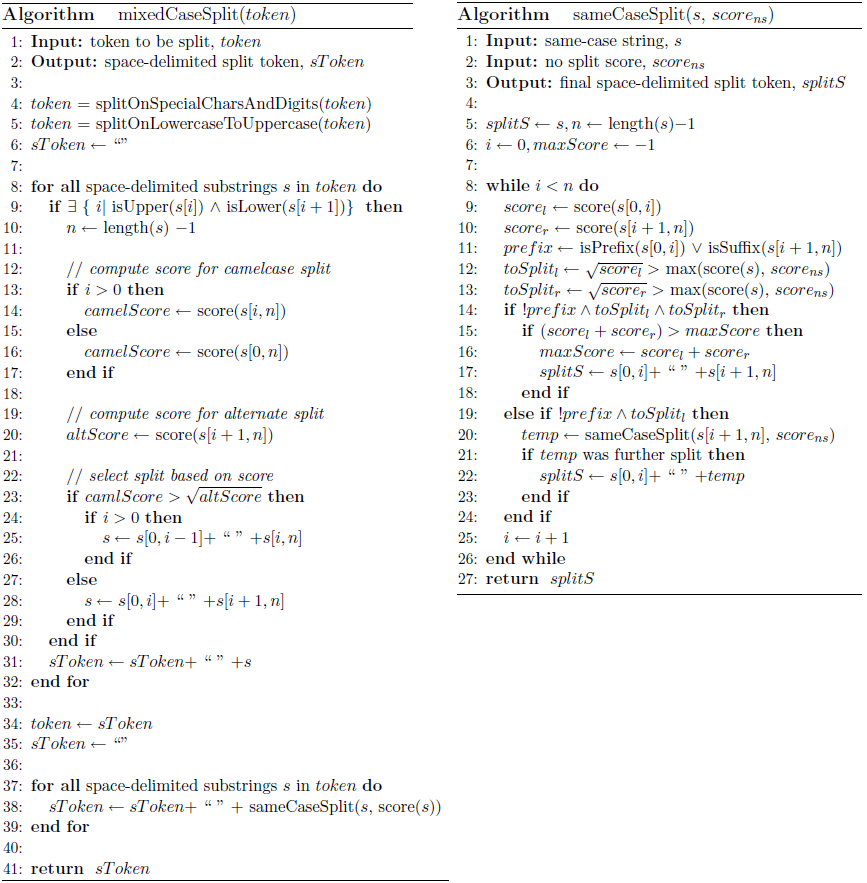
\includegraphics[scale=0.53]{./cap3/sam_1.png}
%\caption{Algoritmos mixedCaseSplit y sameCaseSplit}
%\label{sam1}
%\end{figure}

%aclarar que puede recivir distintos tipos de ids ademas de los ya mencionados
La ejecución del algoritmo Samurai, invoca dos rutinas primero se ejecuta \mbox{\textit{divisiónHardWord}} y después \mbox{\textit{divisiónSoftWord}}. La primera básicamente se encarga de dividir los hardwords (palabras que poseen guión bajo o son del tipo camel-case), luego cada una de las palabras obtenidas (en forma de softword), son pasadas a la segunda rutina para continuar con el análisis. A continuación se explican ambas rutinas.

\noindent \textbf{\\División Hardword\\}

En la rutina \textit{divisiónHardWord} (Ver Algoritmo \ref{AHW}) primero se ejecutan dos funciones (líneas 1 y 2). La primera \textit{dividirCaracteresEspecialesDigitos}, toma al token y reemplaza todos los posibles caracteres especiales y números por espacio en blanco. La segunda \mbox{\textit{dividirMinusSeguidoMayus}}, agrega un blanco entre dos caracteres que sea una minúscula seguido por una mayúscula. En este punto solo quedan tokens de la forma softword o que contengan una mayúscula seguido de minúscula (Ejemplos: \textsf{List, ASTVisitor, GPSstate, state, finalstate, MAX}).

Los casos de softword que se obtuvieron (\textsf{state}, \textsf{finalstate}, \textsf{MAX}) van directo a la rutina \mbox{\textit{divisiónSoftWord}}.
El resto del tipo, mayúscula seguido de minúscula (\textsf{List, ASTVisitor, GPSstate}) continúa con el proceso de división. Con respecto a estos tipos, el autor, hace la siguiente clasificación:

\begin{description}
\itemsep0em%reduce espacio
\item[Camel-case sencillo:] La mayúscula indica el comienzo de la nueva palabra. Ejemplos: \textsf{List}, \textsf{AST Visitor}. 
\item[Variante Camel-case:] El autor a través de estudios de datos, se encontró con variantes en donde la mayúscula indica el fin de una palabra. Ejemplos: \textsf{SQL list}, \textsf{GPS state}.
\end{description}


\begin{algorithm}[t!]
\LinesNumbered%enumera las lineas
\SetKwInOut{Input}{Entrada}\SetKwInOut{Output}{Salida}
\Input{\textbf{\textit{token}} \tcp{\textit{token a dividir}}}
\Output{\textbf{\textit{tokenSep}} \tcp{\textit{token separado con espacios}}}
\BlankLine
\textbf{\textit{token}} $\leftarrow $ dividirCaracteresEspecialesDigitos(\textbf{\textit{token}})

\textbf{\textit{token}} $\leftarrow $ dividirMinusSeguidoMayus(\textbf{\textit{token}})

\textbf{\textit{tokenSep}} $\leftarrow $ “”
\BlankLine
\ForAll{$($\textbf{\textit{s}} $|$ \textbf{\textit{s}} es un substring  separado por ` ' en \textbf{\textit{token}}$)$}{
\BlankLine

\If{$($ $\exists \{ i|esMayus(\textbf{s}[i])  \land  esMinus(\textbf{s}[i+1]) \}$ $)$}{
\BlankLine
$n \leftarrow$ length(\textbf{\textit{s}}) $-$ 1
\BlankLine
\tcp{\textit{se determina con la función score si es del tipo camelcase u otra alternativa}} 
\BlankLine
$scoreCamel \leftarrow$ score(\textbf{\textit{s}}[i,n])   

$scoreAlter \leftarrow$ score(\textbf{\textit{s}}[i+1,n])  
\BlankLine
\If{$(scoreCamel > \sqrt{scoreAlter})$}{
\BlankLine
\If{$($i $>$ 0$)$}{
\BlankLine
\textbf{\textit{s}} $\leftarrow$ \textbf{\textit{s}}[0,i $-$ 1] + ` ' + \textbf{\textit{s}}[i,n] \tcp{\textit{GP Sstate}}
}

}\Else{
\BlankLine
\textbf{\textit{s}} $\leftarrow$ \textbf{\textit{s}}[0,i] $+$ ` ' $+$ \textbf{\textit{s}}[i $+$ 1,n]  \tcp{\textit{GPS state}}
}

}
\BlankLine
\textbf{\textit{tokenSep}} $\leftarrow$ \textbf{\textit{tokenSep}} $+$ ` ' $+$\textbf{\textit{s}}

}
\BlankLine
\textbf{\textit{token}} $\leftarrow$ \textbf{\textit{tokenSep}}

\textbf{\textit{tokenSep}} $\leftarrow$ ` '
\BlankLine
\ForAll{$($\textbf{\textit{s}} $|$ \textbf{\textit{s}} es un substring separado por ` ' en \textbf{token}$)$}{
\BlankLine
\textbf{\textit{tokenSep}} $\leftarrow$ \textbf{\textit{tokenSep}} $+$ ` ' $+$ \textbf{divisiónSoftWord}(\textbf{\textit{s}},score(\textbf{\textit{s}}))
}
\BlankLine
\Return \textbf{\textit{tokenSep}}

\caption{divisiónHardWord \label{AHW}}
\end{algorithm}

El algoritmo para determinar cual es el tipo correcto y no tomar malas decisiones (Ejemplos: \textsf{SQ Llist} o \textsf{GP Sstate}), divide a la palabra por ambas consideraciones (ejemplo: \textsf{GP Sstate} y \textsf{GPS state}), luego calcula el puntaje (score) de la parte derecha de ambas divisiones (líneas 7 y 8). Aquella con puntaje más alto entre las dos será por la cual se decida (línea 9). La raíz cuadrada se explica más adelante. Tomando como ejemplo el id \textsf{GPSstate}, para el caso camel-case calculará \mbox{\textit{score(Sstate)}} y para la otra variante \textit{score(state)}. Intuitivamente, la función score (a través de las tablas de frecuencias de palabras) elegirá \textit{state} sobre \textit{sstate} ya que esta última debería tener un puntaje inferior (frecuencia menor de aparición). Por ende Samurai detecta que \textsf{GPSstate} es del tipo Variante de Camel-Case. La división elegida se lleva a cabo en las líneas 11 y 13 (según el caso).
Finalmente, todas las partes que fueron divididas se envían a \mbox{\textit{divisiónSoftWord} (línea 17, 18)}.

%========================
\noindent \textbf{\\División Softword\\}

La rutina recursiva \textit{divisiónSoftWord} (Ver Algoritmo \ref{ASW}) recibe como entrada un substring \textbf{\textit{s}}, el cual puede tener tres tipos de variantes: a) todos los caracteres en minúsculas (\textsf{visitor}), b) todos con mayúsculas (\textsf{VISITOR}), c) el primer caracter con mayúscula seguido por todas minúsculas (\textsf{Visitor}). El otro parámetro de entrada es el puntaje original (\textbf{\textit{score$_{sd}$}}) \mbox{correspondiente a \textbf{\textit{s}}}.

La rutina primero examina cada punto posible de división en \textbf{\textit{s}} dividiendo en \textbf{\textit{split$_{izq}$}} y \textbf{\textit{split$_{der}$}} respectivamente (líneas 4 y 5). La decisión de cual es la mejor división (línea 9), se basa en: a) substrings que no tengan prefijos o sufijos conocidos, los mismos están disponibles en la página web del autor\footnote[1]{Listas de prefijos y sufijos  http://www.eecis.udel.edu/˜enslen/Site/Samurai.} (línea 6), b) que el puntaje de la división elegida sobresalga del resto de los puntajes (líneas 7-8).

%una sola division no se llama recursivamente (!prefix ^ toSplitl ^ toSplitr)
Para aclarar los puntos a) y b) mencionados en el párrafo precedente, para cada partición (izquierda o derecha) obtenida se calcula el score (líneas 4 y 5). Luego este se compara con el puntaje máximo (\textit{max(..)}) entre el puntaje de la palabra original (\textbf{\textit{score$_{sd}$}}, score original) y el puntaje de la palabra actual (score(\textbf{\textit{s}})). En un principio ambos puntajes serán iguales, ya que se trata de la misma palabra, pero a medida que avance la recursión score(\textbf{\textit{s}}) puede variar con respecto a \textbf{\textit{score$_{sd}$}} (líneas 7 y 8). La raíz cuadrada se explica más adelante.
%agregar ejemplos gráficos etc.

%si se cumple solo la parte izquierda se llama recursivamente (!prefix ^ toSplitl)
El \textsf{si} de la línea 9, controla que no tenga prefijos y sufijos ordinarios, y que la parte derecha e izquierda sean serios candidatos a ser divididos, a su vez, se determina con esto, que la parte derecha es una palabra que no necesita dividirse más. En las líneas 10 y 11 se comprueba que la división se realice siempre y cuando, supere al máximo puntaje obtenido hasta el momento. En la línea 12 procede a separar la palabra.

\begin{algorithm}[t!]
\LinesNumbered%enumera las lineas
\SetKwInOut{Input}{Entrada}\SetKwInOut{Output}{Salida}
\Input{\textbf{\textit{s}} \tcp{\textit{softword string}}}
\Input{\textbf{\textit{score$_{sd}$}} \tcp{\textit{puntaje de s sin dividir}}}
\Output{\textbf{\textit{tokenSep}} \tcp{\textit{token separado con espacios}}}
\BlankLine%espacio en blanco

\textbf{\textit{tokenSep}} $\leftarrow$ \textbf{\textit{s}}, n $\leftarrow$ length(\textbf{\textit{s}}) - 1

i $\leftarrow$ 0, \textbf{\textit{maxScore}} $\leftarrow -$ 1
\BlankLine

\While{$($i $<$ n$)$}{
\BlankLine
\textbf{\textit{score$_{izq}$}} $\leftarrow$ score(\textbf{\textit{s}}[0,i])

\textbf{\textit{score$_{der}$}} $\leftarrow$ score(\textbf{\textit{s}}[i+1,n])
\BlankLine
\textbf{\textit{preSuf}} $\leftarrow$ esPrefijo(\textbf{\textit{s}}[0,i]) $\vee$ esSufijo(\textbf{\textit{s}}[i+1,n])
\BlankLine
\textbf{\textit{split$_{izq}$}} $\leftarrow$  $\sqrt{score_{izq}} >$ max(score(\textbf{\textit{s}}),\textbf{\textit{score$_{sd}$}})

\textbf{\textit{split$_{der}$}} $\leftarrow$  $\sqrt{score_{der}} >$ max(score(\textbf{\textit{s}}),\textbf{\textit{score$_{sd}$}})
\BlankLine

\If{$($!\textbf{\textit{presuf}} $\land$ \textbf{\textit{split$_{izq}$}} $\land$ \textbf{\textit{split$_{der}$}}$)$}{
\BlankLine
\If{$(($\textbf{\textit{split$_{izq}$}} $+$ \textbf{\textit{split$_{der}$}}$)$ $>$ \textbf{maxScore}$)$}{
\BlankLine
\textbf{\textit{maxScore}} $\leftarrow$ (\textbf{\textit{split$_{izq}$}}$+$\textbf{\textit{split$_{der}$}})

\textbf{\textit{tokenSep}} $\leftarrow$ \textbf{\textit{s}}[0,i] + ` ' + \textbf{\textit{s}}[i+1,n]
}

}\ElseIf{$(!$\textbf{\textit{presuf}} $\land$ \textbf{\textit{split$_{izq}$}}$)$}{
\BlankLine
\textbf{\textit{temp}} $\leftarrow$ \textbf{divisiónSoftWord}(\textbf{\textit{s}}[i+1,n],\textbf{\textit{score$_{sd}$}})

\If{$($\textbf{\textit{temp}} se dividió?$)$}{
\textbf{\textit{tokenSep}} $\leftarrow$ \textbf{\textit{s}}[0,i] + ` ' + \textbf{\textit{temp}}
}

}
\BlankLine
i $\leftarrow$ i+1
}
\BlankLine
\Return \textbf{\textit{tokenSep}}

\caption{divisiónSoftWord \label{ASW}}
\end{algorithm}

El \textsf{si} de la línea 13, controla que no tenga prefijos y sufijos ordinarios, y que únicamente la parte izquierda es un candidato serio a ser separado, mientras que la cadena de la parte derecha se invoca recursivamente con la misma rutina \textit{divisiónSoftWord}, porque podría seguir dividiéndose en más partes (línea 14).

Si la parte derecha finalmente se divide (línea 15 - el \textsf{si} es verdadero), luego entre la parte izquierda y la derecha también. Por ejemplo, el \mbox{id \textsf{countrownumber}} primero se analiza \textsf{rownumber} (parte derecha - línea 14) como este finalmente se separará en \mbox{\textsf{row number}}, la palabra \textsf{count} (parte izquierda) se divide del resto (línea 16), dando como resultado \mbox{\textsf{count row number}}. Sin embargo, cuando la parte derecha no se divide tampoco se debería separar entre ambas partes (línea 15 - el \textsf{si} es falso). Los análisis de datos hechos por el autor \cite{EHPV09} obligan a hacer este control, ya que se encontraron abundantes casos erróneos de división, uno de ellos es \textsf{string ified}. Con este nuevo control al no dividirse \textsf{ified} tampoco lo hará del resto dejando la palabra correctamente unida \textsf{stringified}. 


%que no se debe separar la actual posición, en base solo a la evidencia en la izquierda ya que puede ser erróneo, un caso conocido erróneo es \textsf{string ified}. 

%La ejecución recursiva de samurai para la cadena \textsf{nonnegativedecimaltype} se ejecuta correctamente y da como resultado \textsf{nonnegative decimal type} \cite{EHPV09}.

Otro problema detectado son las palabras de pocos caracteres (menor a 3). Estas palabras, tienen mucha aparición en los códigos y por lo general el puntaje es más alto que el resto. Por esta razón, el autor \cite{EHPV09} en base a un análisis sustancial decide colocar la raíz cuadrada en algunos resultados de score antes de comparar (línea 7 y 8), sino la división frecuentemente sería errónea. Un ejemplo es la palabra \mbox{\textsf{per formed}}, esto ocurre por que \textsf{per} tiene un alto puntaje y fuerza la separación.

En el algoritmo anterior \textit{divisiónHardWord}, la presencia de la raíz cuadrada (línea 9), cuando se compara el caso camel-case y el caso alternativo también es para solucionar este mismo problema.

\noindent \textbf{\\Función de Scoring\\}

Para que la técnica Samurai pueda llevar a cabo la tarea de separación de ids, se necesita la función de scoring. Como bien se explicó anteriormente, esta función participa en 2 decisiones claves durante el proceso de división:

\begin{itemize}
\itemsep0em%reduce espacio
\item En la rutina \textit{divisiónHardWord}, para determinar si el la división del id es un caso de camel-case o no (líneas 7 y 8).

\item En la rutina \textit{divisiónSoftWord}, para puntuar las diferentes particiones de substrings y elegir la mejor separación (líneas 4, 5, 7 y 8).
\end{itemize}

Dado un string \textbf{s}, la función \textit{score(\textbf{s})} retorna un valor que indica: i) la frecuencia de aparición de \textbf{s} en el programa bajo análisis, y ii) la frecuencia de aparición de \textbf{s} en un conjunto grande de programas predefinidos. Las tablas de frecuencias de aparición de palabras local y global le brindan información a la función score. La inclusión de la tabla de frecuencias global, está dada porque los programas pequeños en general tienen frecuencias bajas en la tabla local, y a veces, la función score no trabaja correctamente a causa de esto.

La fórmula es la siguiente:

\begin{center}
$Frec(s,p) + ( globalFrec(s) / \log_{10}(totalFrec(p) )$
\end{center}

Donde \textbf{p} es el programa de estudio, $Frec(s,p)$ es la frecuencia de ocurrencia de \textbf{s} en \textbf{p}. La función $totalFrec(p)$, es la frecuencia total de todos los strings en el programa \textbf{p}. La función $globalFrec(s)$, es la frecuencia de aparición de \textbf{s} en una gran conjunto de programas tomados como muestras\footnote[1]{Estos programas son alrededor de 9000 y están escritos en JAVA}. Esta fórmula de score fue desarrollada por los autores de la técnica Samurai \cite{EHPV09}, a través de distintos análisis de datos que se realizaron.


\subsection{Algoritmo de Expansión Básico}
\label{sec:algExpBas}
%noindent elimina sangria
%\noindent \textbf{Algoritmo 1}

El algoritmo de expansión de abreviaturas ideado por Lawrie, Feild, Binkley (mismos autores que la técnica de separación Greedy) \cite{LFBEX07} trabaja con cuatro listas para realizar su tarea:

\begin{itemize}
\itemsep0em%reduce espacio
\item Una lista de palabras (en lenguaje natural) que se construye a partir del código fuente.
\item Una lista de frases (en lenguaje natural) presentes también en el código.
\item Una lista de palabras irrelevantes (stop-list).
\item Diccionario de palabras.
\end{itemize}


La primer lista se confecciona de la siguiente manera, para cada método \textit{m} dentro del código se crea una sub-lista de palabras que se extraen de los comentarios que están antes (comentarios JAVA Doc) o dentro del método \textit{m}. También se incorporan palabras hardwords (camel-case o guión bajo) encontradas en los id ubicados en el código, por ejemplo: del id \textsf{easyCase}, se agregan las palabras \textsf{easy} y \textsf{case} al listado. Las palabras que se agreguen en este listado servirán como candidatas a expandir abreviaturas, por eso antes de agregar una palabra en este listado, se filtra utilizando la lista de palabras irrelevantes (esta lista se explica más adelante), para excluir palabras que no colaboran mucho con la expansión y no brindan mucha información.

La lista de frases también contiene una sub-lista por cada método y se construye con una técnica que extrae frases en lenguaje natural \cite{FFCW01}, el principal recurso son los comentarios y los ids multi-palabras. Este listado de frases se utiliza para expandir acrónimos\footnote[1]{Abreviatura formada por las primeras letras de cada palabra en una frase. Ejemplo gif: Graphics Interchange Format.}, si un id en forma de acrónimo coincide con alguna frase, la misma es considerada como potencial expansión \cite{LOPT00} (Ejemplo: la frase \textsf{file status} es una expansión posible para el id \textsf{fs}).

El listado de palabras irrelevantes y el diccionario, están predefinidos con antelación. El primero está compuesto con palabras relacionadas a artículos/conectores (the, an, or), palabras reservadas del lenguaje de programación que se utilicen (\textsf{while, for, if,} etc.). Además posee palabras que no aportan información importante en la comprensión del código, y que son fácilmente reconocidas por los programadores (esta lista se usa con la misma política que el algoritmo Greedy). Por otro lado, las palabras del diccionario, contiene palabras en lenguaje natural, de diccionarios públicos (similar a utilizado por Greedy).

Una vez que las listas de palabras y frases potenciales se confeccionan, comienza la ejecución del algoritmo. La política que utiliza, es dar prioridad primero a la información extraída del código y más aún, a la cercanía de donde este ubicada la abreviatura a expandir, es decir, se busca primero en la sub-lista correspondiente al método donde se encuentra la abreviatura, luego en el resto de las listas con información extraída del código y por último en el diccionario público.

Este algoritmo (Ver Algoritmo \ref{BEA}) recibe como entrada la abreviatura a expandir y las 4 listas antes descriptas. El primer paso, es ver si la abreviatura forma parte de la lista de palabras irrelevantes (stop-list línea 1 y 2, algoritmo \ref{BEA}), en caso afirmativo finaliza la ejecución, ya que no es importante expandir, en caso negativo continúa la ejecución. En caso de continuar, se chequean si alguna de las frases extraídas del código se correspondan con la abreviatura en forma de acrónimo\footnote[1]{Las letras de la abreviatura coincidan con las primeras letras de cada palabra en la frase. Ejemplo: fs $\Rightarrow$ file system.} (línea 5, algoritmo \ref{BEA}), dando prioridad aquellas que se encuentren cercanas al método (a través de la sub-lista correspondiente).
Si no hubo resultados, la búsqueda prosigue en la lista de palabras recolectadas del código, en este caso las letras de la abreviatura deben coincidir en el mismo orden que las letras de una palabra en la lista (línea 8, algoritmo \ref{BEA}), si esto se cumple, la palabra elegida es una candidata, ejemplos: \mbox{\textsf{horiz}} $\Rightarrow$ HORIZ\textsf{ontal}, \textsf{trg} $\Rightarrow$ TR\textsf{ian}G\textsf{le}. Aquí se emplea la misma política de expansión que la búsqueda anterior, dando la preferencia a las palabras que están cerca del método (a través de la sub-lista correspondiente). 


\begin{algorithm}[h!]
\LinesNumbered%enumera las lineas
\SetKwInOut{Input}{Entrada}\SetKwInOut{Output}{Salida}
\Input{\textit{\textbf{abrev}} \tcp{\textit{Abreviatura a expandir}}}
\Input{\textit{\textbf{listaPalabras}} \tcp{\textit{Palabras extraídas del código}}}
\Input{\textit{\textbf{listaFrases}} \tcp{\textit{Frases extraídas del código}}}
\Input{\textit{\textbf{stopList}} \tcp{\textit{Palabras Excluyentes}}}
\Input{\textit{\textbf{dicc}} \tcp{\textit{\textit{Diccionario en Inglés}}}}
\Output{\textbf{únicaExpansión} \tcp{\textit{Abreviatura expandida, o null}}}
\BlankLine
\BlankLine

\If{$($\textit{\textbf{abrev}} pertenece \textit{\textbf{stopList}}$)$}{
\Return null
}
\BlankLine
listaExpansión $\leftarrow$ [ ]
\BlankLine
\BlankLine
\tcp{\textit{Buscar coincidencia de acrónimo.}}

\ForAll{$($\textit{\textbf{Frase}} $|$ \textit{\textbf{Frase}} es una frase en \textit{\textbf{listaFrases}}$)$}{
\BlankLine

\If{$($\textit{\textbf{abrev}} es un acrónimo de \textit{\textbf{Frase}}$)$}{
\tcp{\textit{Se prioriza aquella Frase que está en el mismo método que abrev}}

\Return \textit{\textbf{Frase}} 
}
}

\BlankLine
\BlankLine
\tcp{\textit{Buscar abreviatura común.}}

\ForAll{$($\textit{\textbf{Pal}} $|$ \textit{\textbf{Pal}} es una palabra en  \textit{\textbf{listaPalabras}} $)$}{
\BlankLine
\If{ $($\textit{\textbf{abrev}} es una abreviatura de \textit{\textbf{Pal}}$)$}{
\tcp{\textit{Se prioriza aquella Pal que está en el mismo método que abrev}} 
\Return \textit{\textbf{Pal}}
}

}

\BlankLine
\BlankLine
\tcp{\textit{Si no hay éxito, buscar en el diccionario.}}

%\If{$($isEmpty$($listaExpansión$))$}{
%\BlankLine
listaCandidatos $\leftarrow$ buscarDiccionario(\textit{\textbf{abrev}},\textit{\textbf{dicc}})
listaExpansión.add(listaCandidatos)
%}


\BlankLine
\textbf{únicaExpansión} $\leftarrow$ null
\BlankLine
\BlankLine
\tcp{\textit{Debe haber un solo resultado, sino no retorna nada.}}

\If{$($length$($listaExpansión$)$ $=$ 1$)$}{
\BlankLine
\textbf{únicaExpansión} $\leftarrow$ listaExpansión[0]
}
\BlankLine
\Return \textbf{únicaExpansión} 

\caption{Expansión Básica \label{BEA}}
\end{algorithm}

Finalmente, en caso no tener éxito, con las palabras extraídas del código, la búsqueda continúa en el diccionario predefinido como último recurso (línea 10, algoritmo \ref{BEA}). Al igual que la búsqueda anterior, una palabra candidata dentro del diccionario es aquella que contenga todas las letras en el mismo orden que la abreviatura a expandir, ejemplo: \mbox{\textsf{rctgl}} $\Rightarrow$ R\textsf{e}CT\textsf{an}GL\textsf{e}. Dado que el diccionario posee muchas palabras, puede retornar más de un resultado posible.

La técnica de expansión descripta en esta sección, devuelve una única expansión potencial para una abreviatura determinada y en caso contrario no retorna un resultado (líneas 11 - 14, algoritmo \ref{BEA}). El motivo de esto, es porque no tiene programado cómo decidir una única opción ante múltiples alternativas de expansión. A esta característica de mejora, los autores lo presentan como trabajo futuro \cite{LFBEX07,EZH08}.

\subsection{Algoritmo de Expansión AMAP}
\label{sec:algAmap}

El algoritmo de expansión de abreviaturas que construyó Emily Hill, Zachary Fry, Haley Boyd \cite{EZH08} conocido como \textit{Automatically Mining Abbreviation Expansions in Programs} (AMAP), además de buscar expansiones potenciales al igual que el algoritmo anterior, también se encarga de seleccionar la expansión que mejor se ajusta en caso de que haya más de un resultado posible. Otra mejora destacable, con respecto al algoritmo previo es que no se necesita un diccionario con palabras en lenguaje natural. Este tipo de diccionarios incluyen demasiadas palabras e implica disponer de un gran almacenamiento. 

Las fuentes de palabras que se utilizan son:
\begin{itemize}
\itemsep0em%reduce espacio
\item Una lista de abreviaturas comunes: Estas abreviaturas se obtienen automáticamente desde distintos programas. También se puede incorporar palabras en forma personalizada.
\item Una lista palabras irrelevantes (stop-list).
\item Una lista de contracciones\footnote[1]{Palabras en inglés que llevan apostrofes, ejemplo: let's.} más comunes.
\end{itemize}

Para agilizar la lectura se asigna el nombre de “palabras largas” a las palabras normales que no están abreviadas y son potenciales expansiones de las abreviadas.

La técnica automatizada AMAP, busca palabras largas candidatas para una palabra abreviada dentro del código, con la misma filosofía que se usa en la construcción de una tabla de símbolos en un compilador.

Se comienza con el alcance estático más cercano donde se examinan sentencias vecinas a la palabra abreviada. Luego gradualmente el alcance estático crece para incluir métodos, comentarios de métodos, y los comentarios de la clase. Si la técnica no encuentra una palabra larga adecuada para una determinada palabra abreviada, la búsqueda continúa mirando todo el programa y finalmente examina las librerías de JAVA SE 1.5. 

Los autores asumen que una palabra abreviada está asociada a una sola palabra larga dentro de un método. No es frecuente que dentro de un método una palabra abreviada posea más de una expansión posible. En caso de que esto se cumpla, se puede cambiar la asunción. Se puede estipular que una palabra abreviada solo tiene una sola expansión posible dentro de los bloques o, en un contexto más reducido, solo dentro de las sentencias de código.

%A continuación, se explica los pasos que ejecuta la herramienta AMAP: 
%\begin{enumerate}
%\itemsep0em%reduce espacio
%\item Como se realiza la búsqueda para encontrar palabras largas candidatas dentro de un método. 
%\item Como se elije entre múltiples alternativas cual es la mejor expansión.
%\item Como se buscan nuevas palabras si el alcance local del método no es suficiente, a través del método EMF (Expansión más Frecuente). 
%\end{enumerate}

El algoritmo AMAP ejecuta los siguientes pasos:

\begin{enumerate}
\itemsep0em%reduce espacio
\item Buscar palabras largas candidatas dentro de un método.
\item Elegir la mejor alternativa de expansión.
\item Buscar nuevas palabras si en el alcance local no es suficiente, utilizando el método EMF (Expansión más Frecuente).
\end{enumerate}

A continuación, se explican cada uno de estos pasos.\\

Comenzando por el paso 1, la búsqueda de las palabras largas contiene dos algoritmos, uno que recibe como entrada palabras abreviadas compuestas por una sola palabra (singulares) y el otro algoritmo se encarga de procesar multi-palabras.\\

\noindent \textbf{Búsqueda por Palabras Singulares\\}

El primer paso para buscar palabras largas consiste en construir una expresión regular con un patrón de búsqueda.  Este patrón se encarga de seleccionar las palabras largas que coincidan con las letras de la palabra abreviada.

Los patrones se construyen a partir de la palabra abreviada, a continuación se detalla cómo se arman estos patrones: 

\begin{description}
\itemsep0em%reduce espacio
\item[Patrón prefijo:] Se construye colocando la palabra abreviada (\textit{\textbf{pa}}) seguida de la expresión regular [a-z]+ \footnote[1]{La expresión [a-z]+ significa, una o más letras entre la a y la z.}. Las palabras que coinciden si o si deberán comenzar con \textit{\textbf{pa}}. La expresión regular queda: \textit{\textbf{pa}}[a-z]+.

Ejemplo: Dada \textit{\textbf{pa}} = \textsf{arg}, el patrón \textsf{arg}[a-z]+ coincide con la palabra \textit{\textbf{arg}}ument (entre otras).

\item[Patrón compuesto por letras:]  La expresión regular se construye insertando [a-z]* \footnote[2]{La expresión [a-z]* significa, cero o más letras entre la a y la z.} después de cada letra de la palabra abreviada (\textit{\textbf{pa}}). Si \textit{\textbf{pa}}$=c_{1},c_{2},c_{3},..,c_{n}$, donde $n$ es la longitud de la palabra abreviada. El patrón queda: $c_{1}$[a-z]*$c_{2}$[a-z]*$c_{3}$[a-z]*..$c_{n}$.

Ejemplo: Dada \textit{\textbf{pa}} = \textsf{pgm}, el patrón \textsf{p}[a-z]*\textsf{g}[a-z]*\textsf{m}[a-z]* coincide (entre otras) con  \textit{\textbf{p}}ro\textit{\textbf{g}}ra\textit{\textbf{m}} (entre otras).
\end{description}


%\begin{figure}[h] %[h] para here [b] para bottom [t] para top
%\centering
%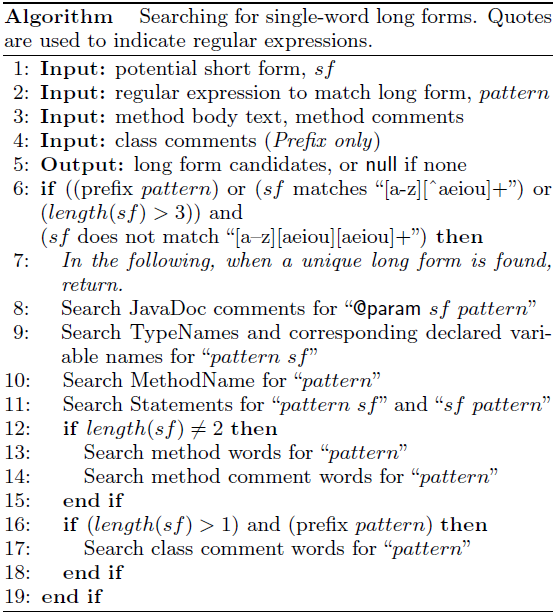
\includegraphics[scale=0.7]{./cap3/exp_1.png}
%\caption{Algoritmo de Expansión de una sola Palabra.}
%\label{exp1}
%\end{figure}

La búsqueda de palabras singulares se presenta en el algoritmo \ref{BPS}. Los parámetros de entrada son: la palabra abreviada a expandir y la expresión regular formada por el patrón elegido.

En la línea 1 (del algoritmo \ref{BPS}), se impide básicamente dos cosas: 

a) Que no se procesen palabras abreviadas con muchas vocales consecutivas (segundo argumento del $\land$ en el \textsf{si}). Este control lo determinaron los autores de AMAP \cite{EZH08}, ya que comprobaron que la mayoría de las palabras abreviadas con vocales consecutivas se expanden como multi-palabras (ejemplos: es el caso de los acrónimos \textsf{gui} $\Rightarrow$ \textsf{graphical user interface}, \textsf{ioe} $\Rightarrow$ \textsf{invalid object exception}). El algoritmo de la próxima sección es el encargado de expandirlos (multi-palabras).

b) En caso de que el patrón sea el \textit{compuesto por letras} (no sea el prefijo), se hacen dos controles más (primer argumento del $\land$ en el \textsf{si}). El primero verifica que la abreviatura no posea muchas vocales consecutivas (“[\^{}aeiou]+” logra eso) y el segundo controla que la longitud sea mayor que 3. Los autores a través del análisis de datos determinaron esta restricción \cite{EZH08}, ya que el \textit{patrón compuesto por letras} tiene el inconveniente que es muy flexible y tiende a capturar muchas palabras largas incorrectas. Por ejemplo: \textsf{lang} $\Rightarrow$ (\textsf{loading}, \textsf{language}), o \textsf{br} $\Rightarrow$ (\textsf{bar}, \textsf{barrier}, \textsf{brown}), entre otros.

En las líneas 2-10 se describe el proceso de búsqueda. Si alguna de estas sentencias de búsqueda encuentra una única palabra larga candidata, el algoritmo finaliza y retorna el resultado. 

\begin{algorithm}[t!]
\LinesNumbered%enumera las lineas
\SetKwInOut{Input}{Entrada}\SetKwInOut{Output}{Salida}
\Input{\textit{\textbf{pa}} \tcp{\textit{Palabra Abreviada}}}
\Input{\textit{\textbf{patrón}} \tcp{\textit{Expresión regular}}}
%\Input{\textit{\textbf{ccMétodo}} \tcp{\textit{Cuerpo y Comentarios del Método}}}
%\Input{\textit{\textbf{comClase}} \tcp{\textit{Comentarios de la Clase}}}
\Output{\textit{\textbf{palCand}} \tcp{\textit{Palabras candidatas, o null si no hay}}}
\BlankLine
\tcp{\textit{Las expresiones regulares están entre comillas}}
\BlankLine

\If{ $($\textbf{patrón} prefijo $\vee$ \textit{\textbf{pa}} coincide “[a-z][\^{}aeiou]$+$” $\vee$ length(\textit{\textbf{pa}}) $>$ 3$)$ $\land$ $($\textit{\textbf{pa}} no coincide con “[a-z][aeiou][aeiou]$+$”$)$}{

\BlankLine
\tcp{\textit{Si alguna de las siguientes búsquedas encuentra un único resultado, el algoritmo lo retorna finalizando la ejecución}}
\BlankLine
Buscar en Comentarios JavaDoc con “\textsf{\at param} \textit{\textbf{pa patrón}}”, si el resultado es único \Return en \textit{\textbf{palCand}}
\BlankLine
Buscar en Nombres de Tipos y la correspondiente Variable declarada con “\textit{\textbf{patrón pa}}”, si el resultado es único \Return en \textit{\textbf{palCand}}
\BlankLine
Buscar en el Nombre del Método con “\textit{\textbf{patrón}}”, si el resultado es único \Return en \textit{\textbf{palCand}}
\BlankLine
Buscar en las Sentencias con “\textit{\textbf{patrón pa}}” y “\textit{\textbf{pa patrón}}”, si el resultado es único \Return en \textit{\textbf{palCand}}
\BlankLine
\If{$($length(\textit{\textbf{pa}}) $\neq$ 2$)$}{
\BlankLine
Buscar en palabras del Método con “\textit{\textbf{patrón}}”, si el resultado es único \Return en \textit{\textbf{palCand}}
\BlankLine
Buscar en palabras que están en los Comentarios del Método con “\textit{\textbf{patrón}}”, si el resultado es único \Return en \textit{\textbf{palCand}}

}

\If{$($length(\textit{\textbf{pa}}) $>$ 1$)$ $\land$ $($\textit{\textbf{patrón}} prefijo$)$}{
\BlankLine
\tcp{\textit{Solo se busca con patrones prefijos}}

Buscar en palabras que están en los Comentarios de la Clase con “\textit{\textbf{patrón}}”, si el resultado es único \Return en \textit{\textbf{palCand}}
}
}

\caption{Búsqueda por Palabras Singulares \label{BPS}}
\end{algorithm}

En la línea 2 la búsqueda se realiza en los comentarios Java Doc, donde la expresión regular es “\at param \textit{\textbf{pa}} \textit{\textbf{patrón}}”. Por ejemplo, si en Java Doc se tiene el comentario “\at param ind index” donde \textit{\textbf{pa}} = \textbf{ind}, \textit{\textbf{patrón}} = \mbox{“ind[a-z]+”}. La expresión regular \mbox{“\at param ind ind[a-z]+”} coincidirá y devolverá el resultado  “index” como expansión de \textbf{ind}.

Si el algoritmo no encuentra resultados, sigue la búsqueda en la línea 3 con los nombres de los tipos ubicados en las variables declaradas, donde la expresión regular es “\textit{\textbf{patrón}} \textit{\textbf{pa}}”. Por ejemplo, si se tiene una declaración “\textbf{component comp}” donde \textit{\textbf{pa}} = \textbf{comp}, \textit{\textbf{patrón}} = “comp[a-z]+”  la expresión regular \mbox{“comp[a-z]+ comp”} coincidirá y devolverá el resultado  “component” como expansión de \textbf{comp}.

Si el algoritmo continúa sin resultados, sigue en la línea 4 donde se busca coincidir con “\textit{\textbf{patrón}}” en el nombre del método. En caso de seguir sin resultados, prosigue en la línea 5 con distintas variantes “\textit{\textbf{patrón}} \textit{\textbf{pa}}” o “\textit{\textbf{pa}} \textit{\textbf{patrón}}” en las sentencias comunes del método. 

%En la figura \ref{exp3} se pueden observar los distintos casos que se describieron.

Si la ejecución continúa sin encontrar resultados, la línea 6 se restringe una búsqueda por palabras que tengan al menos 3 caracteres ya que generalmente aquellas con 2 tienden a ser multi-palabras (Ejemplo: \textsf{fl $\Rightarrow$ file system} / Ver próxima sección). Luego en la línea 7 se busca con \textit{\textbf{patrón}} solamente en palabras del método (ejemplo: para una abreviatura \textsf{setHor} coincide con una llamada a función con el nombre de \textsf{setHorizontal()}). Después en la línea 8 se busca en palabras de comentarios dentro del método con \textit{\textbf{patrón}}.

Para finalizar, en la línea 10 si la palabra abreviada tiene más de un caracter y el patrón es de tipo prefijo, se busca usando (\textit{\textbf{patrón}}) en los comentarios de la clase. En la línea 9 se restringe esta búsqueda, porque los autores sostienen \cite{EZH08}, que buscar con un solo caracter en comentarios implica tener muchos resultados y más aun si el patrón es el compuesto por letras.

\noindent \textbf{\\\\Búsqueda por Multi-Palabras\\}

El algoritmo de búsqueda por multi-palabras a diferencia del explicado anteriormente, expande abreviaturas que contienen dos o más palabras. Algunos ejemplos son: \textsf{gui $\Rightarrow$ graphical user interface, fs $\Rightarrow$ file system}. Como bien se definió en secciones anteriores estas abreviaturas se las conoce con el nombre de acrónimos, que generalmente están conformadas por 2 ó 3 caracteres. El algoritmo anterior intenta detectar este tipo de abreviaturas y no analizarlas para que sea procesado por el multi-palabras.

Al igual que el algoritmo de palabras singulares, el algoritmo de multi-palabras utiliza expresiones regulares conformada por patrones de búsqueda. Los patrones utilizados en las búsquedas multi-palabras se construyen de la siguiente manera:

%Al igual que la búsqueda por palabras singulares, la búsqueda por multi-palabras se va incrementando en el alcance de código hasta encontrar un candidato que coincida con el patrón. Sin embargo, es importante tener en cuenta hasta donde los patrones multi-palabras realizan la búsqueda. Por ejemplo, una abreviatura \textsf{il} puede coincidir con la frase “\textbf{i}t is importante to \textbf{l}imit” en la sentencia anterior donde se encuentra \textsf{il}. Por eso, se preprocesa el texto y los comentarios dentro del método sin ir mas allá de las declaraciones y de los ids propios del método.

%También se dividen los comentarios y los literales strings en frases usando signos de puntuación (?!,;).

%Las abreviaciones como \textsf{val} no se expanden a \textsf{verify and load}, por que las palabras irrelevantes (stop words) se remueven de los comentarios (en este caso \textsf{and}) en el cuerpo del método.


\begin{description}
\itemsep0em%reduce espacio
\item[Patrón acrónimo:] Se elabora colocando la expresión regular [a-z]+[ ]+ \footnote[1]{La expresión [a-z]+[ ]+ significa, una o más letras entre la a y la z, seguido de espacio.}, después de cada letra de la palabra abreviada (\textit{\textbf{pa}}). Si \textit{\textbf{pa}}$=c_{1},c_{2},c_{3},..,c_{n}$, donde $n$ es la longitud de la palabra abreviada. El patrón queda: \mbox{$c_{1}$[a-z]+[ ]+$c_{2}$[a-z]+[ ]+$c_{3}$[a-z]+[ ]+..[a-z]+[ ]+$c_{n}$}. Permite encontrar acrónimos tales como \textsf{pdf} $\Rightarrow$ \textbf{\textit{p}}ortable \textbf{\textit{d}}ocument \textbf{\textit{f}}ormat.

\item[Patrón de Combinación de Palabras:] En este caso el patrón se construye de manera similar al anterior pero se usa la expresión regular [a-z]*?[ ]*? \footnote[2]{La expresión [a-z]*?[ ]*? significa, cero o más letras entre la a y la z, seguido de espacio o no.} después de cada caracter de la palabra abreviada (\textit{\textbf{pa}}). Si \textit{\textbf{pa}}$=c_{1},c_{2},c_{3},..,c_{n}$, donde $n$ es la longitud de la palabra abreviada. El patrón queda: $c_{1}$[a-z]*?[ ]*?$c_{2}$[a-z]*?[ ]*?$c_{3}$[a-z]*?[ ]*?...[a-z]*?[ ]*?$c_{n}$. De esta manera se pueden capturar palabras del tipo \textsf{arg} $\Rightarrow$ \textbf{\textit{a}}ccess \textbf{\textit{r}}i\textbf{\textit{g}}hts, permitiendo más capturas que el patrón anterior.
\end{description}


%\begin{figure}[h] %[h] para here [b] para bottom [t] para top
%\centering
%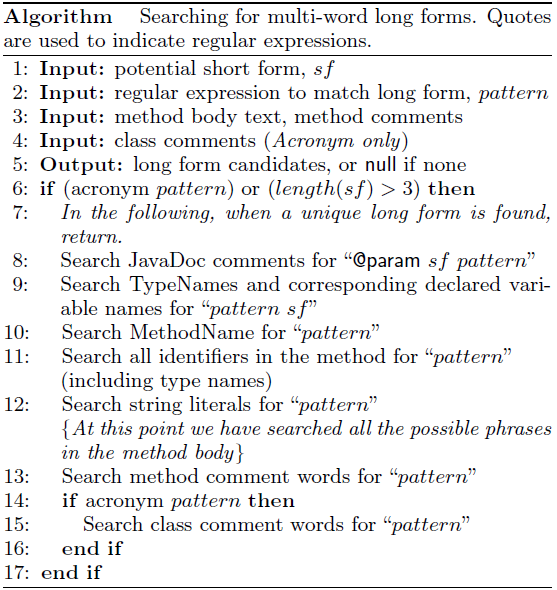
\includegraphics[scale=0.7]{./cap3/exp_2.png}
%\caption{Algoritmo de Expansión Multi-Palabra.}
%\label{exp2}
%\end{figure}

En el algoritmo \ref{BMP}, se presenta la búsqueda por multi-palabras \cite{EZH08}. Las variables de entrada son: la abreviatura multi-palabra a expandir y la expresión regular formada por el patrón elegido.

\begin{algorithm}[t!]
\LinesNumbered%enumera las lineas
\SetKwInOut{Input}{Entrada}\SetKwInOut{Output}{Salida}
\Input{\textit{\textbf{pa}} \tcp{\textit{Palabra Abreviada}}}
\Input{\textit{\textbf{patrón}} \tcp{\textit{Expresión regular}}}
%\Input{\textit{\textbf{ccMétodo}} \tcp{\textit{Cuerpo y Comentarios del Método}}}
%\Input{\textit{\textbf{comClase}} \tcp{\textit{Comentarios de la Clase}}}
\Output{\textit{\textbf{palCand}} \tcp{\textit{Palabras candidatas, o null si no hay}}}
\BlankLine
\tcp{\textit{Las expresiones regulares están entre comillas}}
\BlankLine

\If{$($\textit{\textbf{patrón}} acrónimo $\vee$ length(\textit{\textbf{pa}}) $>$ 3$)$}{

\BlankLine
\tcp{\textit{Si alguna de las siguientes búsquedas encuentra un único resultado, el algoritmo lo retorna finalizando la ejecución}}
\BlankLine
Buscar en Comentarios JavaDoc con “\textsf{\at param} \textit{\textbf{pa patrón}}”, si el resultado es único \Return en \textit{\textbf{palCand}}
\BlankLine
Buscar en Nombres de Tipos y la correspondiente Variable declarada con “\textit{\textbf{patrón pa}}”, si el resultado es único \Return en \textit{\textbf{palCand}}
\BlankLine
Buscar en el Nombre del Método con “\textit{\textbf{patrón}}”, si el resultado es único \Return en \textit{\textbf{palCand}}
\BlankLine
Buscar en todos los ids (y sus tipos) dentro del Método con “\textit{\textbf{patrón}}”, si el resultado es único \Return en \textit{\textbf{palCand}}
\BlankLine
Buscar en Literales String con “\textit{\textbf{patrón}}”, si el resultado es único \Return en \textit{\textbf{palCand}}
\BlankLine
\tcp{\textit{En este punto se buscó en todos los lugares posibles dentro del método}}
\BlankLine
Buscar en palabras que están en los Comentarios del Método con “\textit{\textbf{patrón}}”, si el resultado es único \Return en \textit{\textbf{palCand}}
\BlankLine
\If{$($\textit{\textbf{patrón}} acrónimo$)$}{
\BlankLine
\tcp{\textit{Solo se busca con patrones Acrónimos}}
Buscar en palabras que están en los Comentarios de la Clase con “\textit{\textbf{patrón}}”, si el resultado es único \Return en \textit{\textbf{palCand}}
}
}

\caption{Búsqueda por Multi Palabras \label{BMP}}
\end{algorithm}

Los patrones de \textit{combinación de palabras} son menos restrictivos que los patrones de \textit{acrónimos} y frecuentemente conllevan a malas expansiones. En caso que no sea acrónimo, la búsqueda se restringe a palabras abreviadas ingresadas con longitud 4 ó mayor (línea 1, algoritmo \ref{BMP}). Esto genera la sensación de que se pierden casos de 2 ó 3 caracteres pero estudios indican que son la minoría \cite{EZH08}.
 
Al igual que el algoritmo anterior en las líneas 2-4 se realiza la búsqueda primero en comentarios JAVA Doc, luego en nombres de tipos, después en el nombre del método. La Figura \ref{exp3} muestra algunos ejemplos antedichos.

Dado que las expresiones regulares son más complejas en este algoritmo, los tiempos de respuestas son más elevados. Por esta razón, la búsqueda en sentencias no se realiza, a diferencia del algoritmo de palabras singulares.

\begin{figure}[t] %[h] para here [b] para bottom [t] para top
\centerline{%queda centrada mejor la imagen
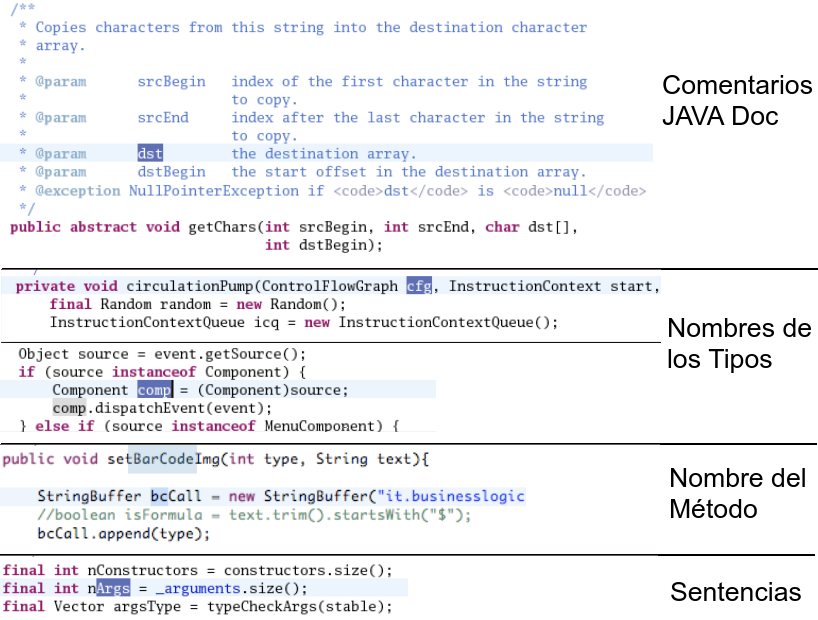
\includegraphics[scale=0.7]{./cap3/exp_3.png}
}
\caption{Ejemplos de distintas Búsquedas dentro del Código}
\label{exp3}
\end{figure}

En las siguientes líneas 5-7 se examinan los ids (incluyendo declaraciones), palabras de literales strings y palabras de comentarios del método. En los tres casos solo se utiliza “\textit{\textbf{patrón}}”.

Luego en la línea 9 se busca en comentarios de la clase con el \textit{patrón acrónimo}. Cabe aclarar que \textit{patrón de combinación de palabras} en este caso no se usa (línea 8) ya que puede tomar palabras largas incorrectas.

Finalmente después de observar cientos de casos de palabras largas, los autores \cite{EZH08} concluyen que el mejor orden de ejecución de las técnicas de búsqueda es ejecutar los patrones: acrónimo (multi-palabra), prefijo (una sola palabra), compuesto por letras (una sola palabra), combinación de palabras (multi-palabra).

Si ninguna de las estrategias de expansión funciona en el ámbito local dentro de un método, se procede a buscar la palabra abreviada en un listado de contracciones (inglés).

En caso de seguir sin éxito, se recurre a la técnica conocida como expansión más frecuente (EMF).
Antes de explicar EMF, esta pendiente describir la forma en que AMAP decide ante varias alternativas de expansión.

\noindent \textbf{\\Decidir entre Múltiples Alternativas\\}

Existe la posibilidad de que una abreviatura posea múltiples alternativas potenciales de expansión, dentro del mismo alcance estático. Por ejemplo, el patrón prefijo para \textsf{val} puede coincidir \textsf{value} o \textsf{valid}. La técnica de elección entre múltiples candidatos procede de la siguiente manera:

\begin{enumerate}
\itemsep0em%reduce espacio
\item Se elije la palabra larga dentro del alcance estático con mayor frecuencia de aparición. Tomando el ejemplo anterior para \textsf{val} si \textsf{value} aparece 3 veces y \textsf{valid} una sola vez, se elije la primera.

\item En caso de haber paridad en el ítem 1, se agrupan las palabras largas con similares características. Por ejemplo, si \textsf{def} coincide con \textsf{defaults}, \textsf{default} y \textsf{define} donde todas aparecen 2 veces, en este caso se agrupa las dos primeras en solo \textsf{default}, sumando la cantidad total a 4 predominando sobre \textsf{define} con 2.

\item En caso de que la igualdad persista, se acumulan las frecuencias de aparición entre las distintas búsquedas para determinar un solo candidato. Por ejemplo, si el id \textsf{fs} coincide con \textsf{file system} y \textsf{file socket} ambas con una sola aparición en los comentarios de JAVA Doc. Para llegar a una decisión, primero se almacenan ambas opciones. Después, prosigue con el resto de las búsquedas (nombres de tipos de ids, literales, comentarios) en cuanto aparezca una de las dos, por ejemplo \textsf{file socket} este termina prevaleciendo sobre \textsf{file system}.

\item Finalmente si todas las anteriores fallan se recurre al método de expansión más frecuente (EMF). 

\end{enumerate}


\noindent \textbf{Expansión Más Frecuente (EMF)\\}


La estrategia EMF \cite{EZH08} es una técnica que se utiliza en 2 casos. Por un lado, 
encuentra una expansión cuando todas las búsquedas fracasan y por el otro, ayuda a decidir entre varias alternativas de expansión. 

La idea consiste en ejecutar la misma estrategia local de expansión de abreviaturas explicada anteriormente, pero sobre el programa entero. Para cada palabra abreviada, se cuenta el número de veces que esa palabra se le asigna una palabra larga candidata. Luego, se calcula la frecuencia relativa de una palabra abreviada con respecto a cada palabra larga encontrada. La palabra larga con mayor frecuencia relativa se considera la expansión más frecuente. Al final del proceso se agrupan las palabras largas potenciales en un listado de EMF.
Sin embargo, suele pasar que la expansión más probable es la incorrecta. Para evitar que esto suceda, una palabra larga debe, a su vez, superar la frecuencia relativa más de la mitad (0.5). Inclusive, la palabra abreviada debe tener al menos 3 asignaciones de palabras largas candidatas en todo el programa.

\begin{table}[b!]
\centering
   \begin{tabular}{| l |l | l |}
     \hline \textbf{Abreviatura} & \shortstack{\textbf{Palabra} \\ \textbf{Expandida}} & \shortstack{\textbf{Frecuencia} \\ \textbf{Relativa}} \\
     \hline int & integer & 0.821 \\
     \hline impl & implement & 0.840 \\
     \hline obj & object & 1.000 \\
     \hline pos & position & 0.828 \\
     \hline	   
   \end{tabular}
   
\caption{Algunas Frecuencias Relativas de Ids en JAVA 5}
\label{tabEmf}
 
\end {table}

La técnica EMF tiene dos niveles de análisis, el primero es a nivel de programa y el otro más general a nivel JAVA. El nivel de programa es ideal ya que expande las abreviaturas con palabras propias del dominio del problema. El nivel más general se arma con la API\footnote[1]{Interfaz de programación de aplicaciones, por su siglas en Inglés.} de JAVA. En la tabla \ref{tabEmf} se muestra algunos casos de frecuencias relativas más altas de JAVA 5. En caso de que una palabra abreviada no obtenga un candidato de expansión, EMF también puede entrenarse sobre muchos programas JAVA para mejorar la precisión. A su vez, existe la posibilidad de armar una lista a mano para casos puntuales de expansión que no son de frecuente aparición. Otras soluciones propuestas son entrenar sobre documentación online relacionada a JAVA o documentación vinculada a la ciencias de computación.
El algoritmo de expansión de abreviaturas AMAP es totalmente automático y se implementó como una extensión de Eclipse. %Actualmente solo soporta procesamiento por lotes. Como trabajo futuro se piensa que corra en segundo plano brindando apoyo a herramientas de mantenimiento de software \cite{EZH08}.\\

%Extracting meaning - lawrie
Hasta ahora se han descripto algoritmos y técnicas que recientemente se pensaron y elaboraron. En la próxima sección se presenta una herramienta que fue construida en los comienzos de los estudios basados en ids. Esta herramienta es tomada como objeto de estudio por varios autores de las técnicas antes mencionadas \cite{EZH08,DCHD06,DLHD06,LFBEX07}.\\


%tonella-caprile
\pagebreak 
\subsection{Herramienta: Identifier Restructuring}
\label{sec:algRest}


\begin{figure}[t!] %[h] para here [b] para bottom [t] para top
\centerline{%queda centrada mejor la imagen
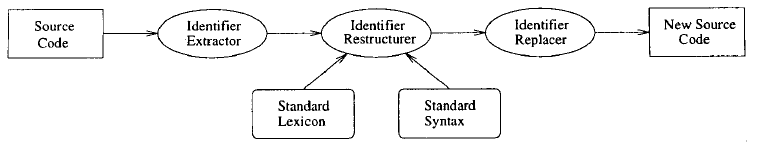
\includegraphics[scale= 0.80]{./cap3/ire_1.png}
}
\caption{Arquitectura de Identifier Restructuring}
\label{ire1}
\end{figure}

La herramienta Identifier Restructuring \cite{BCPT00} se encarga de recibir como entrada un código fuente escrito en lenguaje C. Luego a través de un proceso de transformación cada id del código, se expande a palabras completas. La salida es el mismo código pero con los ids expandidos.
Cabe destacar que esta herramienta es semi-automática, en algunas situaciones necesita intervenir el usuario.

Los ids se cambian por nombres más explicativos, los cuales incluyen un verbo que indica la función del id en el código. Más precisamente después de renombrar los ids, se visualiza claramente el rol que cumple el id en el programa.

El código fuente se convierte de esta manera en un código más claro y mejora la comprensión. El proceso consta de tres etapas (Ver Figura \ref{ire1} \footnote[1]{Todas las figuras de esta sección se obtuvieron del artículo que describe la herramienta Identifier Restructuring \cite{BCPT00}.}): 

\begin{enumerate}
\itemsep0em%reduce espacio
\item \textbf{Identifier Extractor:} Recupera una lista con los nombres de los ids presentes en el código. Este módulo se programó con un parser de lenguaje C, que fue modificado para que reconozca los ids y los extraiga.
\item \textbf{Identifier Restructurer:} Genera una asociación entre el nombre actual del id y un nuevo nombre estándar expandido. El primer paso consiste en segmentar el id en las palabras que lo constituyen. Después, cada palabra se expande usando un diccionario de palabras estándar (estándar léxico). Finalmente, la secuencia de palabras expandidas deben coincidir con reglas predefinidas por una gramática para determinar que acción cumple el id en el código \mbox{(estándar sintáctico).}
\item \textbf{Identifier Replacer:} Transforma el código original en el nuevo código usando las asociaciones que se construyeron en la etapa anterior. Se emplea un scanner léxico para evitar reemplazar posibles nombres de ids contenidos en literales strings y en comentarios.
\end{enumerate}

Los pasos 1 y 3 están totalmente automatizados. Sin embargo, para lograr que la expansión de nombres sea efectiva, se necesita que en algunos casos del paso 2 intervenga el usuario.

\begin{figure}[t!] %[h] para here [b] para bottom [t] para top
\centering
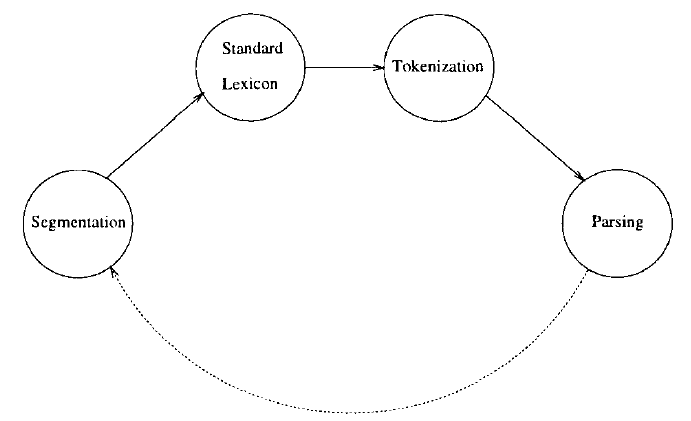
\includegraphics[scale= 0.60]{./cap3/ire_2.png}
\caption{Etapas de Identifier Restructurer}
\label{ire2}
\end{figure}

A continuación, se detalla el paso 2 que es el más importante de esta herramienta, en la Figura \ref{ire2} se desglosa las diferentes etapas.

\begin{description}
\itemsep0em%reduce espacio
\item[Segmentation:] El id se separa en las palabras que lo componen. De manera automática se utilizan estrategias simples de separación (basada en guión bajo o camel-case: hardword - ejemplo: \textsf{get\_txt} $\Rightarrow$ \textsf{get txt}). En caso que existan softwords, la división se debe hacer en forma manual. Por ejemplo: \textsf{get\_txtinput} $\Rightarrow$ \textsf{get txt input} la separación entre \textsf{txt} e \textsf{input} la realiza el usuario. Sin embargo, los autores proponen de manera conceptual (no implementado), utilizar un algoritmo programado (por los mismos autores) en LISP, para detectar y separar casos de softwords \cite{BCPT99}. 

%Este algoritmo utiliza una estrategia Greedy, en donde se va consultado de a un carácter en adelante
%algoritmo hecho en LISP, este toma un string \textit{s} como entrada. Se utiliza una estrategia greedy verificando a partir de la primer letra de \textit{s} un sub-string que pertenezca a un diccionario predefinido. Luego el sub-string se descarta y continúa el análisis con el resto hasta que no haya más sub-strings que separar \cite{BCPT99}.

\begin{figure}[t] %[h] para here [b] para bottom [t] para top
\centerline{%queda centrada mejor la imagen
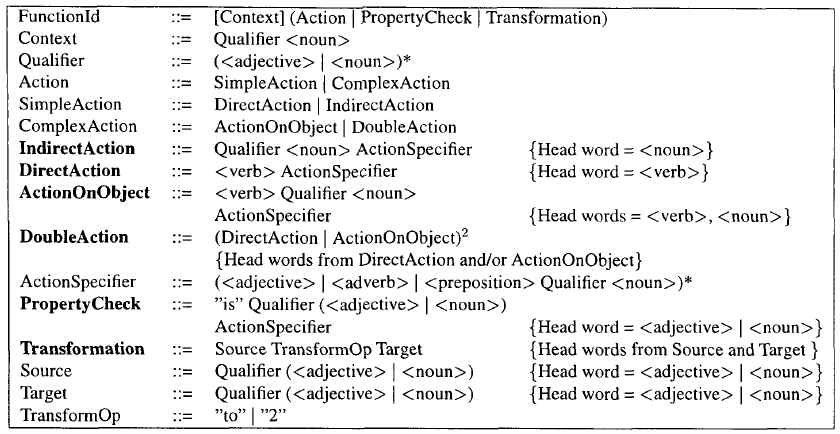
\includegraphics[scale= 0.60]{./cap3/ire_3.png}
}
\caption{Gramática que determina la Función de los Ids}
\label{ire3}
\end{figure}

\item[Standard Lexicon:] Lograda la separación de las palabras estas son mapeadas a una forma estándar (expandidas) con la ayuda de un diccionario léxico \cite{BCPT99} (Ejemplo: \textsf{upd} $\Rightarrow$ \textsf{Update}). Una idea que mejora esta propuesta, es incorporar al diccionario términos extraídos del código fuente. También aquí, el usuario puede intervenir para realizar la expansión manualmente. Los autores de la herramienta construyeron los diccionarios de manera genérica tomando como muestra 10 programas \cite{BCPT00}. Sin embargo, se aconseja que con el tiempo los diccionarios deben crecer con la inclusión de nuevos términos.

\item[Tokenization:] Una vez obtenidas las palabras a una forma estándar (expandidas) en el paso anterior, se procede a asignar cada palabra a un \textit{tipo léxico} (verbo, sustantivo, adjetivo). Por ejemplo, la palabra \textsf{Update} se transforma en $<$Update,verb$>$, \textsf{Standard} a $<$Standard,adjective$>$. Esta tuplas se denominan tokens y se utiliza un `diccionario de tipos' para generarlos de manera automática, este diccionario al igual que los otros se arma previamente a gusto del programador \cite{BCPT99}. Sin embargo, existen casos que se necesita la intervención humana para determinar el tipo correcto. Por ejemplo, \textsf{free} en inglés es un verbo, un adjetivo y a la vez un adverbio.% En este caso la herramienta va a elegir lo que el diccionario le indique (si free esta presente).

\item[Parsing:] Finalmente, la secuencia de tokens obtenidos en la etapa anterior se analiza usando una gramática predefinida. Este análisis permite determinar cuál es el rol/acción del id en el código fuente y de esta manera, se determina la “acción semántica” del id. 
En la Figura 3.8 se muestra un ejemplo de gramática construida por los autores. Cabe aclarar que cada usuario puede elaborar su propia gramática. 
Es una gramática regular donde los símbolos terminales están indicados con $<>$. Las producciones con negrita, determinan en función del tipo léxico asignado a cada palabra la acción semántica del id.
Por ejemplo, el verbo expresa la acción y el sustantivo representa al objeto de la acción, con \textbf{ActionOnObject} $\Rightarrow$ $<$verb$>$,$<$noun$>$ $\equiv$ $<$go,home$>$. Otro ejemplo es, \textbf{IndirectAction} $\Rightarrow$ $<$adjetive$>$,$<$noun$>$ $\equiv$ $<$order,textfield$>$ donde el adjetivo representa una cualidad del sustantivo.

En caso de que el análisis falle el proceso se reinicia desde el comienzo partiendo nuevamente de la etapa de segmentación \cite{BCPT00} (Ver Figura \ref{ire2}).
\end{description}

\begin{figure}[ht] %[h] para here [b] para bottom [t] para top
\centerline{%queda centrada mejor la imagen
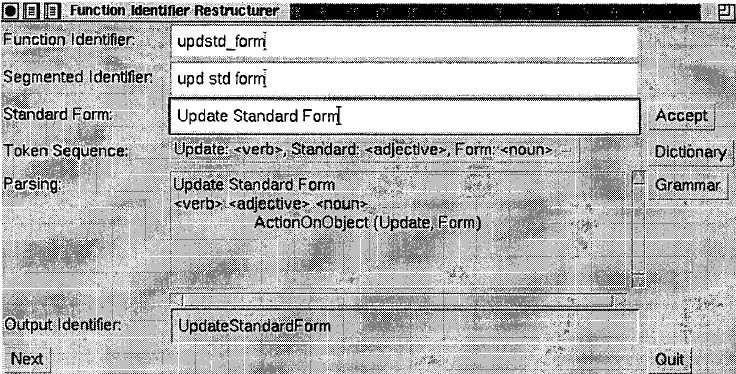
\includegraphics[scale= 0.67]{./cap3/ire_4.png}
}
\caption{Visualización de Identifier Restructuring}
\label{ire4}
\end{figure}

\pagebreak
\noindent \textbf{Interfaz para el Usuario\\}

La interfaz para el usuario de \textbf{Identifier Restructurer} se visualiza en la Figura \ref{ire4}, el id de entrada se muestra en el primer cuadro de texto \textsf{updstd\_form}. Se usan heurísticas sencillas (guión bajo, camel-case) para separar las palabras del id, en este caso \textsf{updstd} y \textsf{form}. Como esta segmentación está incompleta, el usuario puede separar manualmente en el segundo cuadro de texto la palabra \textsf{upd} y \textsf{std} (Ver Figura \ref{ire4}). En el tercer cuadro de texto se propone la forma estándar de cada palabra. Cuando una palabra no se puede expandir la herramienta muestra un signo de pregunta en su lugar (?). En este caso \textsf{upd} $\Rightarrow$ \textsf{Update}, \textsf{std} $\Rightarrow$ (?), \textsf{form} $\Rightarrow$ \textsf{Form}, como \textsf{std} no está presente en el diccionario, se necesita la intervención del desarrollador para que se complete correctamente a \textsf{Standard}. Luego las palabras expandidas son asociadas a la función gramatical. En esta etapa puede existir para una secuencia de palabras más de una función gramatical (la gramática es ambigua y puede generar más de una secuencia de tokens). En caso de suceder esto el usuario puede elegir cual es la secuencia más adecuada. En el ejemplo de la Figura \ref{ire4} solo existe una única función gramatical y es reflejada en el cuarto cuadro de texto. 

Luego, en el cuadro de Parsing (Ver Figura \ref{ire4}) se puede apreciar la acción que aplica el id, en este caso \textbf{ActionOnObject(Update,Form)} `actualizar formulario'. Finalmente el resultado se detalla en el último cuadro de texto de más abajo.

Cuando se arma la asociación de los nombres ids con los nuevos nombres generados la misma debería cumplir con la propiedad de inyectividad, de esta forma se evita que haya conflictos de nombres entre los distintos ids del programa. La herramienta ayuda al programador a conseguir este objetivo resaltando los posibles conflictos en los nombres.

Para concluir con las etapas de esta herramienta, la última fase llamada \textbf{Identifier Replacer} toma todas las ocurrencias del id \textsf{updstd\_form} y se reemplaza por \textsf{UpdateStandarForm}, como se mencionó con anterioridad.

\section{Notas y Comentarios}

Las observaciones que se destacan en el estado del arte de las técnicas de análisis de ids apuntan por un lado, que asignar buenos nombres a los ids ayudan a comprender el sistema. Al comienzo de este capítulo se explicó la herramienta Identifier Dictionary (IDD) que ayuda a lograr este cometido. Sin embargo, no trascendió ya que es costosa de utilizar sobre grandes proyectos de software y solo es efectiva cuando se emplea desde el arranque del desarrollo de un sistema.

La investigación realizada por los autores de IDD, dejaron en claro que los nombres de los ids es crucial para la comprensión de los sistemas, un código con ids más descriptivos y claros se entiende mucho mejor. Además, en este contexto, las herramientas/técnicas de análisis de ids mejoran sus resultados. 
%De esta manera, es más sencillo extraer conceptos del dominio del problema desde los ids.

Con respecto a otras herramientas/técnicas de análisis de ids, las mismas han ido evolucionando con el pasar del tiempo. Al principio algunas etapas necesitaban la intervención del usuario para realizar las tareas, se puede decir que usaban procesos semi-automatizados (ejemplo: \textbf{Identifier Restructurer}). A medida que se construyeron nuevas técnicas, se buscó más la automatización haciendo que el usuario se involucre menos (ejemplo: Samurai, AMAP). 

Habiendo explicado en este capítulo algunas de las estrategias asociadas al análisis de ids en códigos, en el próximo capítulo, se describe una herramienta de análisis de ids que se construyó tomando como referencia algunas de las características propias de las técnicas vistas en este capítulo.

%Como se mencionó en este capítulo, las primeras técnicas utilizaban netamente diccionarios de palabras en lenguaje natural, lo cual requiere mucho espacio de almacenamiento (ejemplo: Greedy). Más tarde, se intentó disminuir el uso de estos diccionarios mirando más los recursos internos de información dentro los sistemas, como es el caso de los comentarios, literales strings y la documentación (ejemplo: Samurai).

%Los autores de las recientes técnicas (Samurai, AMAP) decidieron recurrir a procesos que examinan programas de gran envergadura. Estos procesos recolectan palabras útiles que son almacenadas en forma de listas de palabras. Estos listados no solo ayudan a traducir el significado de los ids, también tiene bajas exigencias de almacenamiento y están constituidos con palabras más adecuadas al ámbito de las ciencias de la computación.


%Con este estudio se puede observar que los ids son una fuente importante de información, por eso elaborar técnicas que analicen ids es un aporte destacado para la CP.

%\section{Técnicas de División de Identificadores}
%\section{Técnicas de Expansión de Identificadores}

%En el área de Ingeniería del Software, existen herramientas automatizadas que permiten hacer análisis de los identificadores utilizados en los códigos de programación. Estas herramientas extraen parcialmente conceptos representados en los identificadores del código fuente para intentar interpretar lo que el programador quiso desarrollar.

%Estas técnicas exhiben información estática oculta detrás de los ids, esta información es importante porque da indicios de lo que un sistema realiza en su ejecución por ende es un aporte en el ámbito de Comprensión de Programas. --colocar abajo